\documentclass[12pt, a4paper]{article}
\setlength{\headheight}{14.49998pt}
\addtolength{\topmargin}{-2.49998pt}

\usepackage{color}
\usepackage{float}
\usepackage{framed}
\usepackage{lineno}
\usepackage{fancyvrb}
\usepackage{siunitx}
\usepackage{amssymb}
\usepackage{amsmath}
\usepackage{microtype}

\setlength{\emergencystretch}{1em}

\usepackage[outputdir=build, cachedir=.minted]{minted}
\setminted{
    fontfamily=tt,
    breaklines=true,
    autogobble=true,
    fontsize=\small,
    bgcolor=codebg
}

\usepackage{fontspec}
\usepackage{enumitem}
\usepackage{polyglossia}

\usepackage{subcaption}
\usepackage{graphicx}
\graphicspath{{img/}}
\usepackage{fancyhdr}
\usepackage{geometry}
\usepackage[colorlinks=true, allcolors=blue]{hyperref}

\usepackage{tikz}
\usetikzlibrary{calc,chains,positioning,shapes.geometric,arrows.meta}

\usepackage{pgfplots}
\pgfplotsset{compat=1.18}


\setmainlanguage{hebrew}
\setotherlanguage{english}

\newfontfamily\hebrewfonttt[Script=Hebrew]{David CLM}
\setmainfont{David CLM}

\setlist[itemize,1]{label={\fontspec{CMU Serif}\textbullet}}
\setlist[itemize,2]{label={\fontspec{CMU Serif}--}}

\definecolor{codebg}{RGB}{245, 245, 245}
\definecolor{schoolgreen}{RGB}{47, 79, 79}

\renewcommand{\listingscaption}{קטע קוד}
\renewcommand{\listoflistingscaption}{רשימת קטעי קוד}

\parskip=0.5em
\linespread{1.15}
\geometry{margin=2.5cm}

\pagestyle{fancy}
\fancyhf{}
\fancyhead[R]{צוף ברזילי}
\fancyhead[L]{\textenglish{AutoScout}}
\fancyfoot[C]{\thepage}
\renewcommand{\headrulewidth}{0.4pt}
\renewcommand{\footrulewidth}{0pt}

\pdfstringdefDisableCommands{%
  \def\textenglish#1{#1}%
}

\begin{document}

\IfFileExists{secrets.tex}{\input{secrets}}{\newcommand{\id}{XXXXXXXXX}}

\begin{titlepage}
\begin{center}

% לוגו בית הספר

\includegraphics[width=0.4\textwidth]{school-logo}

\vspace{2cm}

{\Huge\textbf{פרויקט גמר}}

\vspace{1cm}

{\LARGE\textbf{בנושא:}}

\vspace{0.5cm}

{\LARGE\textbf{\textcolor{schoolgreen}{\textenglish{AutoScout}: מערכת מעקב אוטומטית לרובוטי \textenglish{FRC}}}}

\vspace{2cm}

{\Large
מוגש במסגרת לימודי הנדסת תוכנה\\
התמחות למידת מכונה ולמידה עמוקה\\
\LR{5} יחידות לימוד
}

\vspace{2cm}

\begin{Large}
\begin{tabular}{r@{}l}
\textbf{מגיש/ה:} & \hspace{2cm} צוף ברזילי\\[0.3cm]
\textbf{ת"ז:} & \hspace{2cm} \id\\[0.3cm]
\textbf{מנחה:} & \hspace{2cm} ד״ר שי פרח
\end{tabular}
\end{Large}

\vfill

{\Large \textbf{יוני \LR{2026}}}

\end{center}
\end{titlepage}

\tableofcontents
\newpage

\section{מבוא ותקציר}
\subsection{הבעיה}

בתחרויות \textenglish{FRC} משתתפות בכל מקצה שתי בריתות — כחולה
ואדומה — כאשר בכל ברית שלושה רובוטים של קבוצות שונות. במהלך המשחק כל
רובוט נע במהירות, נבלע לעיתים מאחורי רובוטים אחרים, ומשתנה בזווית
הצילום שלו ביחס למצלמה. כדי לבחור שותפות טובות למקצי הפלייאוף ולבצע החלטות אסטרטגיות אחרות, קבוצות
רבות מבצעות \textenglish{Scouting}: תלמידים צופים במקצים ומזינים ידנית
נתונים על ביצועי הרובוטים.

לשיטה הידנית יש כמה חסרונות בולטים: היא דורשת כוח אדם רב, היא לרוב לא מאפשרת מעקב מלא אחרי מיקומי הרובוטים, והיא רגישה לטעויות אנוש. לכן
נוצר צורך במערכת אוטומטית שתוכל לקבל סרטון וידאו מהיציע, לזהות את כל
הרובוטים במקצה, לעקוב אחרי התנועה שלהם לאורך זמן, ולשייך כל מסלול
לקבוצה הנכונה.

\subsection{הפתרון המוצע}

המערכת שפיתחתי מקבלת כקלט סרטון של מקצה
ומספר מקצה ידוע מראש. מתוך מספר המקצה המערכת יודעת מהן שש הקבוצות
האפשריות שישתתפו בו, ולכן אפשר לצמצם את מרחב החיפוש כבר בתחילת
התהליך. לאחר מכן המערכת פועלת בארבעה שלבים עיקריים:

\begin{itemize}
\item זיהוי כל הרובוטים בפריים באמצעות מודל \textenglish{YOLO}.
\item מעקב אחר כל זיהוי לאורך זמן באמצעות \textenglish{ByteTrack}, כך
  שלכל רובוט נשמר \textenglish{Track ID} יציב ככל האפשר.
\item חיתוך תמונת הרובוט מתוך הפריים והרצת מודל \textenglish{YOLO}
  נוסף לזיהוי הספרות שעל הבאמפר.
\item התאמת כל עקבה למספר קבוצה מתוך שש הקבוצות במקצה בעזרת מנגנון
  ניקוד מצטבר, המשלב את צבע הברית, מרחק
  \textenglish{Levenshtein} ממספרי הקבוצות האפשריים, וסף ביטחון לפני
  קבלת החלטה סופית.
\end{itemize}

פלט המערכת הוא מסלול התנועה המוחלק של כל רובוט לאורך כל המקצה. בצורה זו ניתן לעבור משלב של צפייה ידנית בלבד לשלב של ניתוח
אוטומטי למחצה או אוטומטי מלא של התנהגות הרובוטים לאורך המשחק.

\subsection{פתרונות דומים והייחוד של הפרויקט}

הגישה הנפוצה ביותר כיום בסביבת \textenglish{FRC} היא עדיין סקאוטינג
ידני, שבו תלמידים עוקבים אחרי רובוטים ומזינים נתונים בזמן אמת. קיימות
גם מערכות ראייה ממוחשבת כלליות לזיהוי ומעקב אחר אובייקטים, אך הן בדרך
כלל אינן פותרות לבדן את שאלת הזהות של כל רובוט כאשר כמה רובוטים דומים
זה לזה ומופיעים באותו מגרש.

הייחוד של הפרויקט שלי הוא בשילוב בין כמה מקורות מידע חלשים יחסית,
שביחד יוצרים החלטה חזקה: זיהוי רובוטים, מעקב תנועתי, זיהוי ספרות על
הבאמפר, וצמצום המועמדים האפשריים לפי לוח המשחקים של המקצה. במקום לנסות
לזהות את מספר הקבוצה במדויק בכל פריים בנפרד, המערכת צוברת ראיות לאורך
זמן ומקבלת החלטה רק כאשר הביטחון המצטבר מספיק גבוה.

\subsection{סרטון הדגמה}

יש להוסיף כאן קישור לסרטון הדגמה קצר של המערכת בפעולה
(זיהוי רובוטים, מעקב ושיוך קבוצות): \textbf{[להוסיף קישור]}.

\subsection{סיכום תוצאות}

בבדיקות שביצעתי התקבלו התוצאות העיקריות הבאות:
\begin{itemize}
\item מודל זיהוי הרובוטים השיג \textenglish{mAP@50} של כ־\textbf{0.95}.
\item מודל זיהוי הספרות הגיע לדיוק של כ־\textbf{0.70} ברמת הספרה
  הבודדת.
\item לאחר שילוב זיהוי הספרות עם צבע הברית, לוח המשחקים ואלגוריתם
  \textenglish{Levenshtein}, הדיוק הסופי בשיוך עקבה לקבוצה עלה
  ל־\textbf{[להשלים]}.
\item המערכת מצליחה להפיק עבור כל קבוצה מסלול תנועה רציף, שניתן להציג
  לאחר העיבוד לצורך ניתוח המשחק.
\end{itemize}

שתי תוצאות אלו מדגישות את הרעיון המרכזי של הפרויקט: גם כאשר זיהוי
הספרות לבדו עדיין אינו מושלם, שילוב מושכל של כמה שכבות מידע מאפשר
לשפר משמעותית את ההחלטה הסופית ולקבל מערכת שימושית לסקאוטינג.

\section{הגדרת הבעיה כבעיית למידת מכונה}
המערכת השלמה צריכה לקבל סרטון ממקצה ולהחזיר מסלול חלק של כל רובוט
לאורך המקצה --- המיקום שלו בכל נקודת זמן במרווחים קבועים. בשביל לעשות
את זה, חילקתי את המערכת לשני מודלים:

\subsection{מודל זיהוי הרובוטים}

המודל הזה מקבל פריים מהסרטון, ומחזיר את זיהויי הרובוטים: עבור כל
רובוט, \textenglish{Bounding Box} וסיווג של ברית הרובוט לפי הצבע שלו
--- כחול או אדום.

\subsection{מודל זיהוי הספרות}

המודל הזה מקבל תמונה שחתוכה ל־\textenglish{Bounding Box} של רובוט,
ומזהה את הספרות על הבאמפר לפי הסדר שבו הן מופיעות משמאל לימין.

\section{רקע תיאורטי}
\subsection{רקע כללי בלמידה עמוקה}

למידה עמוקה (\textenglish{Deep Learning}) היא תת־תחום של למידת מכונה
(\textenglish{Machine Learning}), המבוסס על שימוש ברשתות נוירונים
מלאכותיות בעלות שכבות רבות. מטרת המערכת היא ללמוד ייצוגים מורכבים של
נתונים מתוך דוגמאות, ללא צורך בהגדרה ידנית של המאפיינים על ידי המתכנת.

\subsubsection{רשתות נוירונים ותהליך ה־\textenglish{Forward Pass}}

רשת נוירונים היא מודל חישובי השואב השראה מפעולת המוח האנושי. היא בנויה
מצמתים (נוירונים) המאורגנים בשכבות:
\begin{itemize}
\item \textbf{שכבת קלט (\textenglish{Input Layer}):} מקבלת את הנתונים
הגולמיים.
\item \textbf{שכבות חבויות (\textenglish{Hidden Layers}):} שכבות אלו
מבצעות חישובים מתמטיים הכוללים כפל של הקלט ב"משקולות"
(\textenglish{Weights}), הוספת הסטה (\textenglish{Bias}) והפעלת
פונקציית אקטיבציה.
\item \textbf{שכבת פלט (\textenglish{Output Layer}):} מחזירה את תוצאת
המודל.
\end{itemize} תהליך ה־\textbf{\textenglish{Forward Pass}} הוא השלב שבו
המידע זורם מהקלט דרך השכבות השונות עד לקבלת החיזוי הסופי.

\subsubsection{פונקציות אקטיבציה}

פונקציות אקטיבציה מכניסות אי־ליניאריות למודל. ללא אי־ליניאריות, גם רשת
בעלת שכבות רבות הייתה שקולה למודל ליניארי פשוט, ולכן לא הייתה מסוגלת
ללמוד תבניות חזותיות מורכבות.

בפרויקט זה נעשה שימוש בפונקציות אקטיבציה ממשפחת \textenglish{ReLU}
(\textenglish{Rectified Linear Unit}), המוגדרת כך:
\[ f(x) = \max(0, x)
\] פונקציה זו יעילה במיוחד לרשתות עמוקות, משום שהיא פשוטה לחישוב
ומסייעת להפחתת בעיית דעיכת הגרדיאנט (\textenglish{Vanishing
Gradient}).

\subsubsection{תהליך הלמידה ואופטימיזציה}

כדי שהרשת תוכל להשתפר, עליה לעבור תהליך איטרטיבי של למידה המורכב
מהשלבים הבאים:
\begin{itemize}
\item \textbf{פונקציית הפסד (\textenglish{Loss Function}):} פונקציה
המחשבת את גודל הטעות של המודל בסוף ה־\textenglish{Forward Pass}. ככל
שערך ההפסד נמוך יותר, כך המודל מדויק יותר.
\item \textbf{מורד הגרדיאנט (\textenglish{Gradient Descent}):} זוהי
האסטרטגיה המרכזית להקטנת השגיאה. אנו מתייחסים לפונקציית ההפסד כאל
"נוף" הררי ומחפשים את הנקודה הנמוכה ביותר בו. הגרדיאנט (הנגזרת) מסמן
לנו את כיוון העלייה, ולכן אנו צועדים בכיוון ההפוך לו כדי "לרדת" במדרון
לעבר מינימום השגיאה.
\item \textbf{פעפוע לאחור (\textenglish{Backpropagation}):} האלגוריתם
המחשב את הגרדיאנטים בפועל. באמצעות "כלל השרשרת" (\textenglish{Chain
Rule}), הרשת מחשבת את הנגזרת של פונקציית ההפסד ביחס לכל משקולת ברשת,
מהסוף (הפלט) חזרה להתחלה (הקלט).
\item \textbf{אופטימייזר (\textenglish{Optimizer}):} האופטימייזר הוא
הרכיב המבצע את עדכון המשקולות בפועל. בפרויקט זה נעשה שימוש באלגוריתם
\textbf{\textenglish{AdamW}}, המשלב קצב למידה אדפטיבי (התאמת גודל הצעד
לכל משקולת), מומנטום (זיכרון של כיווני העדכון הקודמים) ודעיכת משקולות, מה שמאפשר
למידה מהירה ויציבה יותר.
\end{itemize}

\subsubsection{רגולריזציה, \textenglish{Overfitting}
ו־\textenglish{Underfitting}}

המטרה של אימון רשת איננה רק להגיע לביצועים טובים על דוגמאות האימון,
אלא להשיג \textbf{הכללה} (\textenglish{Generalization}) לנתונים חדשים.

שני מצבים בעייתיים במיוחד הם:
\begin{itemize}
\item \textbf{\textenglish{Overfitting} (התאמת יתר):} המודל לומד היטב
את נתוני האימון, אך מתקשה להכליל לנתונים שלא ראה.
\item \textbf{\textenglish{Underfitting} (התאמת חסר):} המודל פשוט מדי,
או לא אומן מספיק, ולכן אינו מצליח ללמוד גם את הדפוסים הבסיסיים.
\end{itemize}

כדי להתמודד עם \textenglish{Overfitting} משתמשים לעיתים בכמה טכניקות
רגולריזציה:
\begin{itemize}
\item \textbf{\textenglish{Dropout}:} השבתה אקראית של נוירונים בזמן
האימון כדי למנוע הסתמכות יתר על מאפיינים מסוימים.
\item \textbf{\textenglish{Batch Normalization}:} נרמול האקטיבציות
בתוך הרשת, המשפר את יציבות האימון ולעיתים גם את ההכללה.
\item \textbf{\textenglish{Early Stopping}:} עצירת האימון כאשר ביצועי
הוולידציה מפסיקים להשתפר.
\end{itemize}

בפרויקטים של ראייה ממוחשבת גם אוגמנטציה (\textenglish{Data
  Augmentation}) ופיצול נכון של הנתונים למערכי אימון, וולידציה ובדיקה
מסייעים להפחתת התאמת יתר.

\subsection{זיהוי אובייקטים (\textenglish{Object Detection})}

זיהוי אובייקטים הוא משימה בראייה ממוחשבת שבה המודל צריך לענות על שתי
שאלות בו־זמנית: \textbf{מה} מופיע בתמונה, ו\textbf{איפה} הוא מופיע.
בפרויקט שלי משימה זו מופיעה פעמיים: פעם אחת לזיהוי הרובוטים על המגרש,
ופעם נוספת לזיהוי הספרות שעל הבאמפר של כל רובוט.

\subsubsection{ההבדל בין \textenglish{Classification}
ל־\textenglish{Detection}}

במשימת סיווג (\textenglish{Classification}) המודל מקבל תמונה ומחזיר
מחלקה. לעומת זאת, בזיהוי אובייקטים (\textenglish{Detection}) המודל
צריך גם לאתר כל אובייקט בתוך התמונה באמצעות תיבה תוחמת
(\textenglish{Bounding Box}).

בפרויקט שלי ההבדל הזה קריטי, משום שבכל פריים יכולים להופיע כמה רובוטים
במקביל. לכן לא מספיק לדעת שיש בתמונה "רובוט", אלא צריך לדעת היכן נמצא
כל רובוט כדי לעקוב אחריו לאורך זמן ולשייך אותו לקבוצה הנכונה.

\subsubsection{רשתות קונבולוציה (\textenglish{CNN})}

הבסיס למודלי זיהוי מודרניים הוא רשתות קונבולוציה
(\textenglish{Convolutional Neural Networks}). רשתות אלו משתמשות
במסננים (\textenglish{Filters}) הסורקים את התמונה ולומדים לזהות תחילה
מאפיינים פשוטים יחסית, כמו קצוות וקווים, ובהמשך מאפיינים מורכבים יותר,
כמו חלקי אובייקט או צורות שלמות.

פלט הביניים של שכבות הקונבולוציה נקרא \textenglish{Feature
Maps}. לעיתים משלבים גם שכבות \textenglish{Pooling}, שמקטינות את הממד
המרחבי של המפות, מפחיתות עומס חישובי, ומבליטות מאפיינים חשובים.

\subsubsection{ארכיטקטורת \textenglish{YOLO}}

בפרויקט זה נעשה שימוש במודלי \textenglish{YOLO} (\textenglish{You Only
Look Once}), השייכים למשפחת הגלאים החד־שלביים (\textenglish{One-Stage
Detectors}). בניגוד למשפחות ישנות יותר כמו \textenglish{R-CNN}
ו־\textenglish{Faster R-CNN}, שמפרידות בין שלב הצעת אזורים לשלב
הסיווג, \textenglish{YOLO} מבצע את כל החיזוי במעבר יחיד על התמונה. לכן
הוא מתאים במיוחד ליישומים שבהם המהירות חשובה.

נהוג לחלק את הארכיטקטורה לשלושה חלקים:
\begin{itemize}
\item \textbf{\textenglish{Backbone}:} החלק שמחלץ מאפיינים חזותיים מן
התמונה.
\item \textbf{\textenglish{Neck}:} החלק שמחבר מאפיינים מכמה קני מידה,
כדי לאפשר זיהוי של אובייקטים בגדלים שונים.
\item \textbf{\textenglish{Head}:} החלק שמחזיר את התיבות, ציוני
הביטחון והמחלקות החזויות.
\end{itemize}

בפרויקט שלי משתמשים בגישה זו הן לזיהוי רובוטים יחסית גדולים בתוך תמונת
המגרש, והן לזיהוי ספרות קטנות יותר מתוך חיתוכים של רובוט בודד.

\subsubsection{\textenglish{Anchor Boxes} ו־\textenglish{Non-Max
    Suppression}}

אחד הרעיונות המרכזיים במודלי זיהוי קלאסיים הוא \textenglish{Anchor
Boxes}: תיבות ייחוס בגדלים וביחסי ממדים שונים, שמהן המודל לומד לסטות
כדי להתאים את התיבה בפועל לאובייקט האמיתי. גם כאשר בגרסאות חדשות של
מודלים מסוימים קיימות גישות \textenglish{anchor-free}, העיקרון עדיין
חשוב להבנת הדרך שבה מערכות זיהוי מטפלות במיקום ובגודל.

לאחר החיזוי, מודל זיהוי עשוי להחזיר כמה תיבות שונות עבור אותו אובייקט.
לכן נהוג להשתמש ב־\textenglish{Non-Max Suppression (NMS)}, אלגוריתם
שבוחר בדרך כלל את התיבה בעלת ציון הביטחון הגבוה ביותר ומסיר תיבות
נוספות שחופפות לה מעל סף מוגדר.

בפרויקט שלי בחרתי להשתמש ב־\textenglish{YOLO26}, שהוא מודל
\textenglish{end-to-end}. לכן, בניגוד למודלים קלאסיים יותר, הוא יכול
להחזיר זיהוי סופי לכל אובייקט בלי להזדקק לשלב \textenglish{NMS} נפרד.
היתרון המעשי הוא תהליך חישוב פשוט ומהיר יותר, דבר שחשוב במיוחד כאשר
רוצים להריץ את המערכת גם על חומרה חלשה יחסית או על \textenglish{CPU} ולשמור על \textenglish{FPS} גבוה.

\subsubsection{מדדי הערכה: \textenglish{IoU}, \textenglish{Precision},
\textenglish{Recall} ו־\textenglish{mAP}}

כדי להעריך את איכות מודל הזיהוי משתמשים בכמה מדדים מרכזיים:
\begin{itemize}
\item \textbf{\textenglish{IoU (Intersection over Union)}:} יחס בין
שטח החפיפה של התיבה החזויה עם תיבת האמת, לבין שטח האיחוד שלהן. ערך
גבוה יותר מעיד על מיקום מדויק יותר.
\item \textbf{\textenglish{Precision}:} איזה חלק מן הזיהויים שהמודל
החזיר אכן נכונים.
\item \textbf{\textenglish{Recall}:} איזה חלק מן האובייקטים האמיתיים
אכן זוהו על ידי המודל.
\item \textbf{\textenglish{mAP}:} מדד מסכם, המשלב בין דיוק לשליפה
לאורך רמות ביטחון שונות, ונחשב לאחד המדדים המרכזיים בזיהוי אובייקטים.
\end{itemize}

\subsubsection{תיוג נתונים בפורמט \textenglish{YOLO}}

כדי לאמן מודל זיהוי אובייקטים, יש צורך בנתונים מתויגים. בכל תמונה יש
לסמן את מיקום האובייקט באמצעות \textenglish{Bounding Box} ולשייך לו
מחלקה. בפורמט \textenglish{YOLO} נהוג לייצג כל אובייקט באמצעות מזהה
מחלקה וארבעה ערכים מנורמלים: מרכז התיבה על ציר $x$, מרכז התיבה על ציר
$y$, רוחב התיבה וגובהה. בפרויקט זה השתמשתי ב־\textenglish{Roboflow}
לצורך תיוג הנתונים וניהולם.

\subsection{מעקב אובייקטים (\textenglish{Object Tracking})}

לאחר שהמערכת מזהה את הרובוטים בכל פריים בנפרד, יש צורך לקשר בין
הזיהויים לאורך זמן. זהו תפקידו של מעקב אובייקטים: לשמור על זהות עקבית
של אותו אובייקט גם כאשר הוא נע, נבלע מאחורי אובייקט אחר, או משנה את
מיקומו בתמונה.

\subsubsection{ההבדל בין \textenglish{Detection}
ל־\textenglish{Tracking}}

לעומת \textenglish{Detection} שמתייחס לכל פריים בפני עצמו, ולכן "שוכח" את מה
שקרה בפריים הקודם, \textenglish{Tracking} מחבר בין זיהויים
עוקבים ומקצה להם \textenglish{Track IDs} עקביים. בלי שלב המעקב, אפשר
היה לדעת היכן נמצאים הרובוטים בכל רגע, אך אי אפשר היה לדעת איזה רובוט
הוא אותו רובוט שראינו בפריים הקודם.

\subsubsection{מעקב מרובה־אובייקטים ו־\textenglish{Data Association}}

בבעיית \textenglish{Multi-Object Tracking} יש צורך לפתור בכל רגע בעיית
שיוך: איזה זיהוי חדש שייך לאיזו עקבה קיימת. תהליך זה נקרא
\textenglish{Data Association}. האלגוריתם מסתמך בדרך כלל על שילוב של
מיקום, מהירות משוערת, חפיפה בין תיבות ולעיתים גם דמיון חזותי.

בפרויקט שלי שלב זה חשוב במיוחד, משום שעל המגרש יש כמה רובוטים דומים,
ולעיתים הם מצטלבים, מסתירים זה את זה, או נעים במהירות גבוהה.

\subsubsection{\textenglish{ByteTrack} לעומת \textenglish{DeepSORT}}

שתי גישות נפוצות למעקב מרובה־אובייקטים הן:
\begin{itemize}
\item \textbf{\textenglish{DeepSORT}:} משתמש לא רק במיקום ובתנועה, אלא
  גם ב־\textenglish{Re-Identification} — כלומר בחתימה חזותית של
  האובייקט.  הדבר מאפשר התמודדות טובה יותר עם חסימות ארוכות, אך דורש
  חישוב נוסף ומודל חזותי נוסף.
\item \textbf{\textenglish{ByteTrack}:} מתמקד בעיקר בשיוך מבוסס תנועה,
  מיקום וחפיפה בין תיבות, אך באופן חכם מנצל גם זיהויים בעלי ביטחון נמוך.
  תכונה זו מועילה במיוחד במקרים של טשטוש תנועה, חסימה חלקית או זיהוי לא
  מושלם.
\end{itemize}

בפרויקט זה בחרתי ב־\textenglish{ByteTrack}, משום שהוא מספק איזון טוב
בין דיוק לבין מהירות, ומתאים ליישום שבו נדרש עיבוד וידאו יעיל
יחסית. בנוסף, אני חוסך אימון של מודל נוסף, וזיהוי הספרות כבר מבצע
בשבילי את ההתאמה מחדש ולא מתבלבל בין רובוטים דומים וויזואלית.

\subsubsection{\textenglish{ID Persistence}, חסימות
  ו־\textenglish{Re-Identification}}

אחד האתגרים המרכזיים במעקב הוא \textenglish{ID Persistence}: היכולת
לשמור על אותה זהות גם כאשר האובייקט מוסתר זמנית. כאשר רובוט חולף
מאחורי רובוט אחר, האלגוריתם צריך להחליט אם מדובר באותו אובייקט שחזר
להופיע או באובייקט חדש.

מערכות מסוימות פותרות זאת בעזרת \textenglish{Re-Identification}, כלומר
השוואת מאפיינים חזותיים של האובייקט בין הופעות שונות. בפרויקט שלי לא
נעשה שימוש ב־\textenglish{Re-Identification} מלא, משום שהבחירה הייתה
להעדיף פתרון מהיר ופשוט יותר חישובית. במקום זאת, המעקב נשען בעיקר על
התנועה, תוצאות הזיהוי והספרות שעל הבאמפר.

מבחינה תאורטית, מערכות \textenglish{Re-Identification} רבות נשענות על
למידת ייצוגים (\textenglish{Embeddings}) באמצעות \textenglish{Contrastive
Learning} או \textenglish{Triplet Loss}, כך שאובייקטים זהים יהיו קרובים
במרחב התכונות ואובייקטים שונים יהיו רחוקים זה מזה. בפרויקט שלי לא היה
צורך להוסיף רכיב כזה, משום שזיהוי הספרות מספק רמז זהות חזק יותר.

\subsubsection{דרישות \textenglish{FPS} וביצועים בזמן אמת}

במערכת \textenglish{Scouting} המיועדת לנתח וידאו של משחקים, המהירות
היא פרמטר קריטי. אם קצב העיבוד נמוך מדי, המערכת תתקשה להיות שימושית
בזמן אמת או אפילו בעיבוד מהיר לאחר המשחק. לכן יש יתרון למודלים ואלגוריתמים
קלים יחסית, שמסוגלים לעבוד בקצב \textenglish{FPS} גבוה, גם אם הם
מוותרים על חלק מן המורכבות של מודלים כבדים יותר.

זוהי אחת הסיבות המרכזיות לבחירה ב־\textenglish{YOLO}
וב־\textenglish{ByteTrack}: שני הרכיבים האלו תוכננו כך שיוכלו לספק
איזון טוב בין ביצועים לבין מהירות.

\subsubsection{כיוונים עתידיים: \textenglish{AprilTags} וכיול גאומטרי}

המערכת הנוכחית פועלת במישור התמונה הדו־ממדי, כלומר היא מנתחת את תנועת
הרובוטים יחסית לפיקסלים בתמונה. בעתיד ניתן לשלב
\textenglish{AprilTags} — סמנים חזותיים ידועים מראש — כדי לכייל את
המצלמה ולבצע מעבר מקואורדינטות של תמונה לקואורדינטות של המגרש האמיתי.

תוספת כזו עשויה לאפשר מדידה מדויקת יותר של מיקום, מהירות ומסלולים על
גבי המגרש עצמו, ולא רק בתוך מסגרת התמונה. עם זאת, היא דורשת תנאי צילום
מתאימים וכיול מצלמה, ולכן נחשבת לכיוון עתידי ולא לרכיב הכרחי במערכת
הנוכחית.

\section{כלים וסביבות פיתוח}
בפרק זה יפורטו כלי התוכנה, הספריות ותשתיות הפיתוח ששימשו לבניית
המערכת. הבחירה בכלים אלו נעשתה מתוך שיקולים הנדסיים של ביצועים בזמן
אמת, קלות תחזוקה ויכולת פריסה כשרת מרכזי.

\subsection{סביבות עבודה ותשתית חומרה}

בשל הבדלי המשאבים הנדרשים בין
שלב האימון לשלב ההרצה, נעשה שימוש בשתי סביבות נפרדות:
\begin{itemize}
\item \textbf{סביבת אימון (\textenglish{Cloud GPU}):} אימון מודלי
  ה־\textenglish{YOLO} בוצע על גבי פלטפורמת \textbf{\textenglish{Google
      Colab}} תוך שימוש במעבד גרפי (\textenglish{GPU}) \textenglish{T4} של חברת
  \textenglish{NVIDIA}. שימוש זה אפשר לקצר משמעותית את זמן האימון של
  הרשתות העמוקות.
\item \textbf{סביבת הרצה ובדיקה (\textenglish{Local CPU}):} בדיקת
  המערכת והרצת השרת בוצעו על מחשב מקומי בעל מעבד \textenglish{Intel
    i7-10700}. סביבה זו מדמה את תנאי העבודה האמיתיים בתחרות, בהם לא תמיד
  קיימת גישה למשאבי ענן חזקים.
\end{itemize}

\subsection{שפות תכנות, \textenglish{Frameworks} וניהול גרסאות}

כדי לעמוד בדרישות הפרויקט מבחינת ביצועים, ניידות ותחזוקה, נעשה שימוש
בכמה שכבות פיתוח שונות:
\begin{itemize}
\item \textbf{שפות תכנות:} צד השרת, עיבוד הוידאו והרצת המודלים פותחו
  ב־\textenglish{Python}, בעוד שממשק המשתמש פותח ב־\textenglish{Dart}
  באמצעות \textenglish{Flutter}.
\item \textbf{\textenglish{Frameworks}:} מודלי הזיהוי הורצו באמצעות
  \textenglish{Ultralytics} על גבי \textenglish{PyTorch}, השרת מומש
  באמצעות \textenglish{FastAPI} והאפליקציה נבנתה במסגרת
  \textenglish{Flutter}.
\item \textbf{ניהול גרסאות:} לאורך הפיתוח נעשה שימוש ב־\textenglish{Git}
  לניהול הקוד, מעקב אחרי שינויים וחזרה לגרסאות קודמות במקרה הצורך.
\end{itemize}

\subsection{ספריות ליבה ועיבוד נתונים (\textenglish{Backend})}

המערכת
מבוססת על שפת \textenglish{Python} ומשתמשת בספריות הבאות:
\begin{itemize}
\item \textbf{\textenglish{Ultralytics}}: המעטפת המרכזית להרצת
  מודלי ה־\textenglish{YOLO} בפורמט \textenglish{PyTorch}.
\item \textbf{\textenglish{Levenshtein}}: ספרייה לחישוב מהיר של
  מרחק עריכה בין מחרוזות. היא משמשת כמרכיב קריטי בתיקון שגיאות זיהוי של
  מספר הקבוצה על ידי השוואת הפלט למספרי הקבוצות המשתתפות במקצה.
\item \textbf{\textenglish{OpenCV} ו־\textenglish{SciPy}}: לניהול
  זרם הוידאו, גזירת תמונות (\textenglish{Crops}) והפעלת מסננים סטטיסטיים
  להחלקת מסלולי הרובוטים.
\item \textbf{\textenglish{NumPy}}: לניהול המטריצות של התמונות
  וביצוע חישובים מספריים על מיקומי האובייקטים.
\end{itemize}

\subsection{תשתית השרת (\textenglish{Infrastructure})}

כדי לאפשר עיבוד
וידאו כבד בסביבת אינטרנט, נעשה שימוש בכלים המאפשרים מקביליות וביצועים
גבוהים:
\begin{itemize}
\item \textbf{\textenglish{FastAPI} ו־\textenglish{Uvicorn}}: השרת
  מבוסס על \textenglish{FastAPI} ורץ על גבי מנוע
  \textenglish{Uvicorn}. בחירה זו מאפשרת טיפול מהיר בבקשות
  \textenglish{HTTP} והעלאת קבצים בצורה יעילה.
\item \textbf{\textenglish{asyncio}}: שימוש בתכנות אסינכרוני
  (\textenglish{Asynchronous Programming}) המאפשר לשרת לנהל מספר פעולות
  במקביל. תשתית זו קריטית כדי לאפשר למשתמשים לבדוק סטטוס עיבוד בזמן
  שהמעבד עסוק בחישוב המודלים.
\end{itemize}

\subsection{ממשק המשתמש (\textenglish{Frontend})}

האפליקציה פותחה
ב־\textbf{\textenglish{Flutter}} (שפת \textenglish{Dart}) תוך שימוש
בחבילות ייעודיות המבטיחות חוויית משתמש חלקה:
\begin{itemize}
\item \textbf{\textenglish{dio}}: לניהול בקשות
  ה־\textenglish{HTTP} והעברת סרטוני הוידאו מול השרת.
\item \textbf{\textenglish{media\_kit}}: חבילה מתקדמת להצגת וידאו
  וניגון מדיה ביציבות גבוהה על גבי מכשירים שונים.
\item \textbf{\textenglish{file\_picker}}: המאפשרת למשתמש לבחור את
  סרטוני המקצים מתוך זכרון המכשיר בצורה נוחה.
\end{itemize}

\subsection{תיוג נתונים וניהול מודלים}

לצורך יצירת מערך הנתונים, נעשה
שימוש בפלטפורמת \textbf{\textenglish{Roboflow}}. הכלי שימש לתיוג ידני
של הספרות, ביצוע אוגמנטציה (\textenglish{Augmentation}) וייצוא
הנתונים בפורמטים המתאימים לאימון.

\subsection{ריכוז הכלים וסביבות הפיתוח}
בשל ריבוי הספריות והכלים בהם נעשה שימוש, ריכזתי את הפירוט הטכני המלא בטבלה \ref{tab:tools_full} המופיעה בנספח \ref{app:tools}.


\section{מערך הנתונים}
\subsection{עקרונות ושיטות בעיבוד הנתונים}

לפני הזנת הנתונים למודלים, כל התמונות עוברות סדרה של פעולות עיבוד
מקדים (\textenglish{Preprocessing}) ואוגמנטציה
(\textenglish{Augmentation}). מטרת שלב זה היא לשפר את יכולת ההכללה
(\textenglish{Generalization}) של המודל ולהבטיח יציבות במהלך האימון.

\begin{itemize}
\item \textbf{נרמול (\textenglish{Normalization}):} תמונות הקלט
  מורכבות מפיקסלים בטווח [0, 255]. כחלק מהעיבוד המוקדם, כל ערכי
  הפיקסלים מחולקים ב־255 כדי להעביר אותם לטווח [0, 1]. פעולה זו קריטית
  למניעת תופעת הגרדיאנטים המתפוצצים (\textenglish{Exploding
    Gradients}), שבה ערכי קלט גבוהים גורמים לעדכוני משקולות קיצוניים
  המונעים מה־\textenglish{Optimizer} להתכנס למינימום בצורה
  יציבה. הנרמול מאפשר למידה מהירה ועקבית יותר.
  
\item \textbf{אוגמנטציה (\textenglish{Data Augmentation}):} כדי
  להתמודד עם כמות נתונים מוגבלת ומגוון תנאי צילום אפשריים (תאורה
  משתנה, זוויות שונות, טשטוש תנועה), השתמשתי בטכניקות אוגמנטציה. פעולה
  זו "מייצרת" דגימות חדשות מתוך הקיימות על ידי שינויים גאומטריים
  ואופטיים, מה שמאלץ את הרשת ללמוד מאפיינים עמידים
  (\textenglish{Robust Features}) ולא להסתמך על רעשי רקע.
\end{itemize}

\subsection{מודל זיהוי הרובוטים}

השתמשתי
ב\href{https://universe.roboflow.com/main-wcgiu/robot-detection-xru6m/16}{מערך
  נתונים} קיים מ־Roboflow, עם מעל 1000 תמונות משידורים רשמיים של
\textenglish{FIRST}. כל רובוט מסומן ב־\textenglish{Bounding Box} שלו
ומסווג לפי הברית שלו: כחול או אדום.

\begin{itemize}
  \item \textbf{אוגמנטציה:} על הנתונים יש אוגמנטציה שמכפילה את מספר תמונות האימון
  פי 3 כדי להגדיל את כמות הנתונים ולהוסיף גיוון כהכנה לתנאי צילום שונים:
  \begin{english}
    \begin{itemize}
    \item \textbf{Shear:} \qty{+-10}{\degree} Horizontal, \qty{+-10}{\degree} Vertical
    \item \textbf{Brightness:} \qty{+-20}{\percent}
    \item \textbf{Noise:} $\leq$ \qty{0.1}{\percent}
    \end{itemize}
  \end{english}

\item \textbf{עיבוד מקדים (\textenglish{Preprocessing}):} התמונה נמתחת
  לגודל של \textenglish{640x640}. התמונה נשארת צבעונית כדי לאפשר את
  סיווג הברית, ועוברת נרמול לטווח [0, 1] על ידי \textenglish{YOLO}.
  
\item \textbf{פיצול הנתונים:} הנתונים פוצלו למערכי אימון, ולידציה
  ובדיקה בחלוקה של
  \textenglish{\qty{75}{\percent}--\qty{15}{\percent}--\qty{10}{\percent}}
  בהתאמה.
\end{itemize}

\subsection{מודל זיהוי הספרות}

השתמשתי
ב\href{https://app.roboflow.com/new-workspace-pyain/nums-llmwb/13}{מערך
  נתונים} עם כ-500 תמונות של רובוטים שתייגתי ידנית בעזרת
\textenglish{Roboflow}. כל ספרה מסומנת ב־\textenglish{Bounding Box}
שלה ומסווגת. התמונות המוקדמות יותר נאספו ונחתכו ידנית ממקורות שונים
כולל סרטונים באיכות גבוהה יותר, בעוד שהמאוחרות יותר נחתכו אוטומטית על
ידי מודל זיהוי הרובוטים מסרטונים רשמיים כדי לדמות את הקלט האמיתי
שהמודל יקבל.

תיוג הנתונים במערך זה לקח כשעתיים.

\begin{itemize}

\item \textbf{אוגמנטציה:} על הנתונים יש אוגמנטציה שמכפילה את מספר תמונות האימון
  פי 3, כדי להגדיל את כמות הנתונים ולהוסיף גיוון כהכנה לתנאי צילום
  שונים, לרובוטים שמופיעים בזוויות שונות ולחיתוכים לא מדויקים של הרובוט:
  \begin{english}
    \begin{itemize}
    \item \textbf{Crop:} $\leq$ \qty{10}{\percent}
    \item \textbf{Rotation:} \qty{+-5}{\degree}
    \item \textbf{Shear:} \qty{+-10}{\degree} Horizontal,
      \qty{+-5}{\degree} Vertical
    \item \textbf{Brightness:} \qty{+-15}{\percent}
    \item \textbf{Exposure:} \qty{+-10}{\percent}
    \end{itemize}
  \end{english}

\item \textbf{עיבוד מקדים (\textenglish{Preprocessing}):} התמונה
  מוגדלת לגודל של \textenglish{128x128} באמצעות
  \textenglish{Letterboxing} (הוספת שוליים שחורים לשמירה על יחס
  גובה־רוחב). התמונה נשארת צבעונית כדי לאפשר זיהוי טוב ופשוט יותר של הבאמפר
  (שעליו הספרות) ועוברת נרמול לטווח [0, 1] על ידי \textenglish{YOLO}.

\item \textbf{פיצול הנתונים:} בגלל הכמות הקטנה יחסית, הנתונים פוצלו
  למערכי אימון, ולידציה ובדיקה בחלוקה של
  \textenglish{\qty{85}{\percent}--\qty{10}{\percent}--\qty{5}{\percent}}
  בהתאמה.
\end{itemize}

\subsection{דוגמאות מתוך מערך הנתונים}

כדי להמחיש את איכות התיוג ואת השונות בנתונים, צורפו דוגמאות ויזואליות
למערכי הנתונים (איורים \ref{fig:robots_sample} ו־\ref{fig:digits_sample}) בנספח
\ref{app:data_samples}.

\subsection{התפלגות מחלקות}

מערך הנתונים כולל איזון בין רובוטים מהברית הכחולה לאדומה, ודגימות של
כל הספרות (0--9) במגוון זוויות צילום ותנאי תאורה, כדי להבטיח הכללה
(\textenglish{Generalization}) טובה של המודל.

להלן התפלגויות הדגימות בשני מערכי הנתונים. ניתן לראות כי המערך מאוזן
יחסית, מה שמסייע במניעת הטיות (Bias) של המודל.

\begin{figure}[H]
  \centering
  \begin{minipage}{0.4\textwidth}
    \centering
    \begin{tikzpicture}
      \begin{axis}[
        width=0.8\textwidth,
        scale only axis,
        ybar,
        xlabel={\texthebrew{מחלקה}},
        ylabel={\texthebrew{כמות}},
        symbolic x coords={כחול, אדום},
        xtick=data,
        ymin=0,
        nodes near coords,
        ]
        \addplot coordinates {(כחול, 3701) (אדום, 3776)};
      \end{axis}
    \end{tikzpicture}
    \caption{התפלגות המחלקות של מודל הרובוטים.}
  \end{minipage}
  \hfill
  \begin{minipage}{0.4\textwidth}
    \centering
    \begin{tikzpicture}
      \begin{axis}[
        width=0.8\textwidth,
        scale only axis,
        ybar,
        xlabel={\texthebrew{מחלקה}},
        ylabel={\texthebrew{כמות}},
        symbolic x coords={0, 1, 2, 3, 4, 5, 6, 7, 8, 9},
        xtick=data,
        ymin=0,
        nodes near coords,
        ]
        \addplot coordinates {(0, 178) (1, 293) (2, 140) (3, 175) (4, 221) (5, 179) (6, 183) (7, 124) (8, 130) (9, 162)};
      \end{axis}
    \end{tikzpicture}
    \caption{התפלגות המחלקות של מודל הספרות.}
  \end{minipage}
\end{figure}

\section{ארכיטקטורת המערכת}
בפרויקט זה לא נבנתה רשת עצבית אחת שמקבלת סרטון ומחזירה מיד את זהות כל
הרובוטים. במקום זאת, פותחה מערכת רב־שלבית המשלבת ממשק משתמש, שרת
עיבוד, שני מודלי זיהוי, אלגוריתם מעקב ומנגנון החלטה דטרמיניסטי.

\subsection{מבט־על על המערכת}

המערכת פועלת כצינור עיבוד סדרתי, שבו כל שלב מוסיף רובד מידע חדש ומצמצם
את אפשרויות הזיהוי, עד לקבלת החלטה דטרמיניסטית. בתרשים הבא ניתן לראות
את מבנה זרימת הנתונים בין הרכיבים השונים במערכת:

\begin{figure}[H]
  \centering
\begin{tikzpicture}[
  node distance=1.2cm and 1.5cm,
  base/.style={draw=black!70, thick, rectangle, rounded corners, align=center, font=\small, minimum height=0.8cm, inner sep=8pt},
  input/.style={base, fill=blue!10},
  model/.style={base, fill=green!10},
  logic/.style={base, fill=orange!10},
  data/.style={base, fill=yellow!15},
  output/.style={base, fill=purple!10},
  arrow/.style={-{Stealth[scale=1.2]}, thick, draw=black!80}
  ]

  \node (video) [input] {\texthebrew{קלט: סרטון וידאו} \\ \textenglish{(Full Match Feed)}};
  \node (yolo_robot) [model, below=of video] {\texthebrew{\textenglish{YOLO26}: זיהוי רובוטים} \\ \texthebrew{וסיווג בריתות}};
  \node (bytetrack) [model, below=of yolo_robot] {\texthebrew{ByteTrack: מעקב אובייקטים} \\ \textenglish{(Track IDs)}};

  \node (matchnum) [input, left=of video, xshift=-1.2cm] {\texthebrew{קלט: מספר מקצה}};
  \node (matchinfo) [data, below=of matchnum] {\texthebrew{שליפת קבוצות המקצה} \\ \textenglish{(Match Schedule Lookup)}};
  
  \node (yolo_digits) [model, right=of bytetrack, xshift=1.5cm] {\texthebrew{\textenglish{YOLO26}: זיהוי ספרות} \\ \texthebrew{(חיתוכי באמפרים)}};
  
  \node (voting) [logic, below=of bytetrack, yshift=-0.5cm] {\texthebrew{מנגנון הצבעה וזיהוי קבוצה} \\ \textenglish{(Levenshtein + Voting + Match Schedule)}};
  \node (smoothing) [logic, below=of voting] {\texthebrew{אינטרפולציה והחלקה גאוסית}};
  \node (final) [output, below=of smoothing] {\texthebrew{פלט: מסלולים מוחלקים} \\ \texthebrew{תצוגת \textenglish{Replay} באפליקציה}};

  \draw [arrow] (video) -- (yolo_robot);
  \draw [arrow] (yolo_robot) -- (bytetrack);

  \draw [arrow] (bytetrack.east) -- (yolo_digits.west)
    node[midway, above, font=\tiny] {\texthebrew{גזירת תמונות}};

  \draw [arrow] (yolo_digits.south) |- (voting.east)
    node[near start, right, font=\tiny, xshift=5pt] {\texthebrew{ספרות חזויות}};

  \draw [arrow] (bytetrack) -- (voting)
    node[midway, left, font=\tiny] {\texthebrew{נתוני מעקב}};

  % חצים של מספר המקצה ולוח המשחקים
  \draw [arrow] (matchnum) -- (matchinfo);
  \draw [arrow] (matchinfo.south) |- (voting.west)
    node[pos=0.25, left, font=\tiny] {\texthebrew{שש קבוצות אפשריות}};

  \draw [arrow] (voting) -- (smoothing);
  \draw [arrow] (smoothing) -- (final);

\end{tikzpicture}
  \caption{תרשים זרימת הנתונים במערכת.}
  \label{fig:system_pipeline}
\end{figure}

התרשים מתאר את זרימת הנתונים המרכזית במערכת בזמן הרצה. מבחינת המימוש
בפועל, ההרצה מתחילה באפליקציית \textenglish{Flutter}, שבה המשתמש בוחר
סרטון מקצה ומזין את מספר המקצה. האפליקצייה שולחת את הסרטון ואת מספר
המקצה לשרת \textenglish{FastAPI}, שמבצע את עיבוד הווידאו ואת כל שלבי
ה־\textenglish{inference}.

בשלב הראשון, השרת משתמש במספר המקצה כדי לשלוף את שש הקבוצות הרלוונטיות
מהלו"ז, שלוש לכל ברית. שימוש זה בידע מוקדם מצמצם את מרחב החיפוש מאלפי
קבוצות אפשריות לשש קבוצות בלבד, ומאפשר למערכת לשלב בין זיהוי חזותי
לבין מידע דומייני זמין מתחרות \textenglish{FRC}.

לאחר מכן הסרטון מעובד פריים אחר פריים. בכל פריים מופעל מודל
\textenglish{YOLO} לזיהוי רובוטים ולסיווג צבע הברית. תיבות הזיהוי
מועברות ל־\textenglish{ByteTrack}, שמחבר בין זיהויים בפריימים עוקבים
ויוצר \textenglish{Track ID} לכל רובוט לאורך זמן. עבור עקבות שעדיין
לא שויכו לקבוצה, השרת גוזר את אזור הרובוט ומפעיל עליו מודל
\textenglish{YOLO} נוסף לזיהוי הספרות שעל הבאמפר.

תוצאות זיהוי הספרות אינן משמשות כהחלטה מיידית על סמך פריים יחיד.
במקום זאת, הן מועברות לשכבת החלטה שמחברת בין צבע הברית, רשימת הקבוצות
במקצה, התאמת \textenglish{Levenshtein} והצבעה מצטברת לאורך זמן. שכבה
זו אחראית להפוך זיהויים חלקיים ורועשים להחלטה יציבה יותר לגבי זהות
הקבוצה של כל עקבה.

בסיום עיבוד הסרטון, המערכת מאגדת את נקודות המיקום של כל קבוצה, מבצעת
אינטרפולציה והחלקה, ומחזירה לאפליקצייה מבנה נתונים המתאר את מסלולי
הרובוטים לאורך המקצה. האפליקצייה משתמשת בפלט זה כדי להציג
\textenglish{Replay} אינטראקטיבי, כולל אפשרות לגלילה בציר הזמן ולהצגת
המסלולים מעל הסרטון המקורי.

ניתן לראות את המערכת כמחולקת לשלוש שכבות: שכבת הראייה הממוחשבת, שכבת
המעקב והשיוך, ושכבת הפלט ועיבוד המסלולים.

\subsection{מדריך למפתח: מבנה הקוד והרצת המערכת}

\subsubsection{מבנה כללי ומיפוי רכיבים לקוד}

מדריך המפתח מתבסס על תרשים זרימת הנתונים שהוצג באיור
\ref{fig:system_pipeline}. בעוד שהתרשים מציג את המערכת ברמת
הארכיטקטורה, חלק זה מתאר כיצד אותם רכיבים ממומשים בפועל בקבצי הקוד,
וכיצד ניתן להריץ את המערכת בסביבת פיתוח מקומית. בפרויקט הנוכחי, רוב
לוגיקת ה־\textenglish{backend} מרוכזת בקובץ \textenglish{main.py},
ולכן המיפוי מתייחס בעיקר לפונקציות המרכזיות בקובץ זה.

\begin{table}[H]
\centering
\begin{tabular}{|p{0.30\textwidth}|p{0.28\textwidth}|p{0.32\textwidth}|}
\hline
\textbf{רכיב} & \textbf{מימוש} & \textbf{תפקיד} \\ \hline

ממשק ושרת &
\textenglish{frontend/}, \textenglish{upload()}, \textenglish{status()} &
שליחת סרטון ומספר מקצה, יצירת משימת עיבוד וקבלת סטטוס. \\ \hline

Pipeline מרכזי &
\textenglish{process()}, \textenglish{run\_pipeline()} &
הרצת כל שלבי העיבוד על הסרטון והחזרת התוצאה הסופית. \\ \hline

זיהוי ומעקב &
\textenglish{model.track()}, \textenglish{frc\_bytetrack.yaml} &
זיהוי רובוטים וצבעי ברית, וחיבור זיהויים לאורך זמן בעזרת \textenglish{ByteTrack}. \\ \hline

OCR ושיוך קבוצות &
\textenglish{detect\_digits()}, \textenglish{update()} &
זיהוי ספרות מחיתוכי רובוטים, צבירת ראיות ושיוך עקבות לקבוצות. \\ \hline

פלט ו־Replay &
\textenglish{smooth\_and\_interpolate()} &
החלקת המסלולים והכנת מבנה נתונים להצגה באפליקצייה. \\ \hline

\end{tabular}
\caption{מיפוי בין רכיבי המערכת לבין המימוש בקוד.}
\end{table}

הטבלה אינה מפרטת כל פונקציה בקוד, אלא מציגה את הקשר בין שלבי המערכת
העיקריים לבין המימוש שלהם.

\subsubsection{מבנה תיקיות וקבצים מרכזיים}

הפרויקט מחולק לשתי תיקיות עיקריות: ה־\textenglish{backend} מרוכז
בתיקייה אחת, וה־\textenglish{frontend} הוא פרויקט
\textenglish{Flutter} נפרד. בתיקיית השורש נמצא גם
\textenglish{Makefile} שמאפשר להריץ את שני הרכיבים במקביל בזמן פיתוח.

\begin{english}
\begin{verbatim}
autoscout/
  Makefile

  backend/
    main.py
    requirements.txt
    start.sh
    frc_bytetrack.yaml

    models/
      robots-*.pt
      digits-*.pt

  frontend/
    ...
\end{verbatim}
\end{english}

שמות קובצי המודלים כוללים את סוג המשימה, גודל המודל ותאריך האימון.
לדוגמה, קובץ בשם \textenglish{robots-nano\_26\_05\_04.pt} מייצג מודל
לזיהוי רובוטים בגודל \textenglish{nano}, שאומן ב־4 במאי 2026. מבנה
שמות זה שימש במהלך הפיתוח כדי לעקוב אחרי גרסאות שונות של מודלים
וניסויים.

\begin{table}[H] \centering
  \begin{tabular}{|p{0.3\textwidth}|p{0.6\textwidth}|} \hline
    \textbf{רכיב} & \textbf{תפקיד} \\ \hline
    \textenglish{backend/main.py} & קובץ השרת המרכזי. כולל את טעינת
    המודלים, קבלת הווידאו, עיבוד הפריימים, הרצת \textenglish{YOLO},
    מעקב עם \textenglish{ByteTrack}, שיוך לקבוצות והחזרת תוצאות. \\
    \hline \textenglish{backend/models/} & תיקייה שבה נשמרים מודלי
    ה־\textenglish{YOLO} המאומנים: מודל זיהוי רובוטים ומודל זיהוי
    ספרות. \\ \hline
    \textenglish{backend/frc\_bytetrack.yaml} & קובץ הגדרות \textenglish{ByteTrack} שהותאם למעקב אחרי רובוטי \textenglish{FRC}. \\ \hline
    \textenglish{backend/requirements.txt} & רשימת ספריות \textenglish{Python} הנדרשות להרצת השרת. \\ \hline
    \textenglish{backend/start.sh} & סקריפט נוחות להפעלת השרת עם \textenglish{uvicorn}. \\ \hline
    \textenglish{frontend/} & פרויקט \textenglish{Flutter} שמציג את ממשק המשתמש: העלאת סרטון, מעקב אחרי עיבוד וצפייה ב־\textenglish{Replay}. \\ \hline
    \textenglish{Makefile} & מאפשר להריץ את ה־\textenglish{backend} ואת ה־\textenglish{frontend} במקביל מתוך תיקיית הפרויקט הראשית. \\ \hline
  \end{tabular}
  \caption{קבצים ותיקיות מרכזיים בפרויקט.}
\end{table}

\subsubsection{הרצת המערכת}

ניתן להריץ את רכיבי המערכת בנפרד, או להשתמש ב־\textenglish{Makefile}
להרצה משולבת בזמן פיתוח.

\noindent\textbf{הרצת ה־Backend}

בהרצה ראשונה יש ליצור סביבת \textenglish{Python} וירטואלית ולהתקין את
התלויות:

\begin{english}
\begin{verbatim}
cd backend
python -m venv .venv
source .venv/bin/activate
pip install -r requirements.txt
\end{verbatim}
\end{english}

לאחר האתחול הראשוני, ניתן להפעיל את השרת באמצעות סקריפט הנוחות:

\begin{english}
\begin{verbatim}
backend/start.sh
\end{verbatim}
\end{english}

הסקריפט עובר אוטומטית לתיקיית \textenglish{backend}, מפעיל את הסביבה
הווירטואלית \textenglish{.venv}, ומריץ את שרת ה־\textenglish{FastAPI}
באמצעות \textenglish{uvicorn} על פורט \textenglish{8000}.

\noindent\textbf{הרצה משולבת}

\begin{english}
\begin{verbatim}
make dev
\end{verbatim}
\end{english}

פקודה זו נועדה לנוחות בזמן פיתוח, והיא מפעילה את ה־\textenglish{backend}
ואת ה־\textenglish{frontend} במקביל. בפועל ניתן להריץ כל רכיב גם בנפרד.

\subsubsection{הערות מימוש ותחזוקה}

הקובץ \textenglish{frc\_bytetrack.yaml} מבוסס על הגדרות ברירת המחדל של
\textenglish{ByteTrack}, אך עבר התאמות למשימת המעקב אחרי רובוטים
בסרטוני \textenglish{FRC}. מטרת ההתאמות היא לשפר את יציבות
ה־\textenglish{Track IDs} במצבים של תנועה מהירה, חסימות חלקיות
ורובוטים שנמצאים קרוב זה לזה.

בגרסה הנוכחית של הפרויקט, רוב לוגיקת ה־\textenglish{backend} מרוכזת
בקובץ \textenglish{main.py}. מבנה זה נבחר משום שהמערכת ממוקדת יחסית:
קבלת סרטון, עיבודו, הרצת מודלי הזיהוי, מעקב, שיוך קבוצות והחזרת
פלט. ריכוז הקוד בקובץ אחד הקל על פיתוח מהיר, בדיקות ושינויים תכופים
במהלך העבודה.

בגרסה עתידית ניתן לשפר את תחזוקת הקוד על ידי פיצול
\textenglish{main.py} למודולים נפרדים, למשל:
\textenglish{inference.py} לטעינת המודלים והרצתם,
\textenglish{tracking.py} לניהול \textenglish{ByteTrack},
\textenglish{team\_assignment.py} לשכבת ההצבעה והשיוך,
ו־\textenglish{video\_processing.py} לעיבוד הווידאו.

\subsection{שכבת הראייה הממוחשבת}



מודל זיהוי הרובוטים מבוסס על ארכיטקטורת \textenglish{YOLO26n} ומודל
זיהוי הספרות על \textenglish{YOLO26s}. אלה מודלי ה־\textenglish{nano}
וה־\textenglish{small} --- הקטנים ביותר --- בסדרה החדשה ביותר של
\textenglish{YOLO}: בזכות כמות הפרמטרים הקטנה מתאפשרים ביצועים מהירים
גם על חומרה חלשה יותר, ובזכות מבנה ה־\textenglish{end-to-end} של סדרת
\textenglish{YOLO26}, אין צורך בשלב \textenglish{NMS} כחלק מהזיהוי, מה
שמשפר את המהירות אפילו יותר. בשביל מודל זיהוי הספרות נבחר מודל קצת
גדול יותר כי הוא מאפשר דיוק גבוה יותר בלי פגיעה משמעותית במהירות, כי
בין הספרות יש יותר מחלקות ויותר קושי להבדיל ביניהן.

בפרויקט זה נעשה שימוש בשני מודלים נפרדים המבוססים על ארכיטקטורת
\textenglish{YOLO26}. הטבלה הבאה מסכמת את ההבדלים המבניים והתפעוליים
ביניהם:

\begin{table}[H]
\centering
\caption{השוואת מפרט טכני: זיהוי רובוטים לעומת זיהוי ספרות.}
\label{tab:model_comparison}
\begin{tabular}{|l|c|c|}
\hline \textbf{מאפיין} & \textbf{מודל זיהוי הרובוטים} & \textbf{מודל
זיהוי הספרות} \\ \hline \textenglish{Base Model} &
\textenglish{YOLO26n} (Nano) & \textenglish{YOLO26s} (Small) \\ \hline
גודל קלט & $3 \times 640 \times 640$ & $3 \times 128 \times 128$
\\ \hline פרמטרים & 2.4M & 9.5M \\ \hline
שכבות & כ־122 & כ־329 \\ \hline \textenglish{FLOPs} & 5.4B & 5.18B
\\ \hline
\end{tabular}
\end{table}

הבחירה ב-\textenglish{YOLO26n} עבור זיהוי הרובוטים נועדה לאפשר קצב
פריימים גבוה בזמן אמת על תמונת המקור המלאה, בעוד שהשימוש
ב-\textenglish{YOLO26s} על קלט קטן ($128 \times 128$) אפשר דיוק גבוה
יותר בזיהוי הספרות תוך ניצול העובדה שהקלט כבר חתוך וקטן משמעותית.

\subsection{שכבת המעקב והשיוך}

\subsubsection{מעקב באמצעות \textenglish{ByteTrack}}

לאחר שלב הזיהוי, המערכת מפעילה \textenglish{ByteTrack} כדי לקשר בין
התיבות בפריימים עוקבים. כך, במקום להתייחס לכל זיהוי כאל אירוע נפרד,
המערכת בונה עקבות רציפות בזמן. לכל עקבה נשמר \textenglish{Track ID},
ובהמשך גם היסטוריית מיקומים של מרכז התיבה.

הבחירה ב־\textenglish{ByteTrack} מתאימה במיוחד לפרויקט זה, משום שהיא
מספקת איזון טוב בין מהירות לדיוק, ויכולה לעבוד היטב גם כאשר חלק מן
זיהויי הרובוטים חלשים יחסית. זה חשוב בסרטוני תחרות, שבהם יש טשטוש תנועה,
חסימות חלקיות ושינויים חדים בכיוון.

\subsubsection{מנגנון ההצבעה המצטבר}

החלק הייחודי ביותר בארכיטקטורה הוא שכבת ההחלטה. לכל \textenglish{Track
ID} נשמר וקטור ניקוד באורך 6, אחד לכל קבוצה אפשרית במקצה. בכל פעם
שמתקבל זיהוי ספרות חדש, המערכת מחשבת ניקוד חדש משני מקורות מידע:

\begin{itemize}
\item \textbf{צבע הברית:} אם הרובוט זוהה כברובוט כחול, רק שלוש הקבוצות
  של הברית הכחולה מקבלות יתרון, ולהפך עבור ברית אדומה.
\item \textbf{דמיון למספרי הקבוצות:} הספרות שזוהו מושוות לכל אחת משש
  הקבוצות במקצה. מכיוון שמודל ה־OCR עלול לטעות בספרה אחת עקב רעש
  ויזואלי או הסתרה, לא ניתן להסתמך על השוואת מחרוזות בינארית (נכון/לא
  נכון). במקום זאת, השתמשתי באלגוריתם מרחק לוינשטיין
  (\textenglish{Levenshtein Distance}), המחשב את מספר הפעולות המינימלי
  הנדרש להמרת מחרוזת אחת לאחרת. המרחק מנורמל, כך שמתקבלת החלטה רציפה —
  לדוגמה, זיהוי "3318" במקום "3316" יקבל ניקוד גבוה בזכות דמיון
  חלקי. פתרון זה מעניק למערכת חוסן (\textenglish{Resilience}) מפני
  שגיאות זיהוי נקודתיות.
\end{itemize}

במימוש הנוכחי שני מקורות המידע משוקללים באופן שווה, ולאחר מכן מעודכנים
בממוצע מעריכי לאורך הזמן. המשמעות היא שהחלטה סופית אינה מבוססת על פריים
בודד, אלא על הצטברות עקבית של ראיות. כך, אם זיהוי ספרות אחד שגוי, הוא
לא מפיל מייד את השיוך של העקבה כולה.

בנוסף, המערכת אוכפת אילוץ חד־חד־ערכי: בכל רגע קבוצה אחת יכולה להיות
משויכת רק לעקבה פעילה אחת. לכן, כאשר נשקל שיוך חדש, נלקחות בחשבון רק
קבוצות פנויות או קבוצות שהעקבה שלהן הוגדרה כ"אבודה" זמנית על ידי
העוקב.

\subsubsection{קבלת החלטה, סף ביטחון ומרווח דינמי}

שיוך סופי אינו מתקבל אוטומטית עבור המועמד בעל הניקוד הגבוה ביותר. כדי
לאשר זהות, המערכת דורשת שני תנאים: שהניקוד של המועמד המוביל יעבור סף
מינימלי, ושיהיה פער מספיק בינו לבין המועמד השני.

המרווח הזה אינו קבוע. אם שתי קבוצות במקצה בעלות מספרים דומים מאוד,
לדוגמה מספרים שנבדלים בספרה אחת בלבד, גם זיהוי ספרות טוב עשוי לתת
ניקוד דומה לשתי הקבוצות. לכן המרווח הנדרש בין המועמד המוביל לבין
המועמד השני מותאם לדמיון בין מספרי הקבוצות במקצה, שנמדד גם הוא באמצעות
\textenglish{Levenshtein} מנורמל.

כאשר מספרי הקבוצות שונים מאוד זה מזה, המערכת דורשת פער גדול יותר בין
המועמד הראשון לשני, משום שצפוי שיהיה קל יותר להבחין ביניהם. לעומת זאת,
כאשר מספרי הקבוצות דומים מאוד, המערכת מסתפקת בפער קטן יותר, משום שגם
זיהוי נכון עשוי להניב ציונים קרובים. עם זאת, המערכת עדיין דורשת
שהניקוד של המועמד המוביל יעבור סף מינימלי, ולכן לא מתקבלת החלטה על סמך
ראיה חלשה בלבד.

קטע הקוד לשלבי ההצבעה וקבלת ההחלטה צורף בקטע קוד
\ref{lst:voting_system} בנספח \ref{app:listings}.

\subsubsection{טיפול בחסימות ובהחלפת זהויות}

בסרטוני תחרות רובוטים נוטים לחצות זה את זה, להסתיר זה את זה ואף לצאת
לרגע מן הפריים. כדי לצמצם שגיאות זהות, המערכת מפעילה שני מנגנוני הגנה:

\begin{itemize}
\item אם עקבה שהייתה משויכת לקבוצה נעלמת ואינה נמצאת עוד בין העקבות
  הפעילות או האבודות, השיוך שלה משתחרר.
\item אם שתי עקבות שכבר קיבלו שיוך נראות כמי שחצו זו את זו בין שני
  פריימים עוקבים, המערכת מבטלת זמנית את האישור לשתיהן ומאפסת את ההצבעה,
  כדי למנוע מצב של החלפת זהויות שקטה.
\end{itemize}

מנגנונים אלו אינם מושלמים, אך הם משקפים בחירה ארכיטקטונית חשובה:
להעדיף מערכת שמסוגלת לחזור למצב של אי־ודאות ולבנות מחדש ביטחון, במקום
להיצמד לזהות שגויה לאורך זמן.

\subsection{שכבת הפלט ועיבוד המסלולים}

במהלך כל הריצה נשמר עבור כל \textenglish{Track ID} רצף של מיקומים,
המיוצג על ידי מרכז תיבת התיחום בכל חותמת זמן. לאחר מכן, ברגע שיש שיוך
לקבוצה, המערכת מאגדת יחד את כל קטעי העקבה המתאימים לאותה קבוצה, גם אם
במהלך המשחק הזהות בוטלה ואושרה מחדש.

כדי להפיק פלט שימושי לניתוח, מתבצעים שלושה שלבים נוספים:

\begin{itemize}
\item \textbf{איחוד ומיון כרונולוגי:} כל הנקודות של אותה קבוצה נאספות
  וממוינות לפי זמן.
\item \textbf{אינטרפולציה:} המסלול נדגם מחדש בקצב קבוע של
  \textenglish{\qty{50}{\Hz}}, כדי לקבל ייצוג אחיד ורציף.
\item \textbf{החלקה:} מופעל מסנן גאוסי חד־ממדי על צירי $x$ ו־$y$ כדי
  לצמצם רעש ולייצר מסלול חלק יותר לצפייה ולניתוח.
\end{itemize}

הפלט הסופי של השרת הוא מבנה נתונים הכולל את שמות הקבוצות, משך הסרטון,
גודל הפריים ורשימת נקודות עבור מסלול כל קבוצה. האפליקצייה משתמשת במידע
זה כדי להציג \textenglish{Replay}  אינטראקטיבי של המקצה, עם אפשרות להניח את המסלולים גם
מעל הווידאו המקורי.

\subsection{שיקולי תכנון והצדקה ארכיטקטונית}

הבחירה בארכיטקטורה זו נבעה מכמה שיקולים עיקריים:

\begin{itemize}
\item \textbf{ניצול ידע דומייני:} מספר המקצה מספק מידע חזק מאוד, ולכן
  חבל להתעלם ממנו ולפתור את הבעיה כאילו כל קבוצות \textenglish{FRC}
  הן מועמדות אפשריות בכל רגע.
\item \textbf{פירוק בעיה קשה לתת־בעיות פשוטות יותר:} זיהוי רובוטים,
  זיהוי ספרות, מעקב ושיוך הם אתגרים שונים. טיפול נפרד בכל אחד מהם מקל על
  האימון, על הניתוח ועל איתור שגיאות.
\item \textbf{עמידות לרעש:} זיהוי הספרות ברמת פריים בודד אינו מספיק
  אמין, ולכן נדרש מנגנון צבירת ראיות לאורך זמן במקום סיווג מיידי.
\item \textbf{יעילות חישובית:} מודל הספרות רץ רק על חיתוכים של עקבות
  שטרם קיבלו שיוך, ולא על כל רובוט בכל פריים, וכך נחסך זמן חישוב.
\item \textbf{הפרדה בין ממשק לעיבוד:} חלוקה ללקוח \textenglish{Flutter}
  ולשרת \textenglish{FastAPI} מאפשרת עיבוד אסינכרוני של סרטונים בלי
  לחסום את חוויית המשתמש.
\end{itemize}

לסיכום, ארכיטקטורת המערכת בפרויקט זה מבוססת על העיקרון של
\textbf{שילוב כמה רמזים חלשים להחלטה חזקה אחת}. במקום להסתמך על מודל
יחיד שיפתור את כל הבעיה בבת אחת, המערכת מחברת בין זיהוי, מעקב, ידע
מוקדם ולוגיקה של החלטה — וכך משיגה פתרון מעשי יותר לבעיית הסקאוטינג
האוטומטי.

\section{תהליך האימון}
\subsection{אסטרטגיית האימון}

בפרויקט זה לא אומנה מערכת אחת מקצה לקצה, אלא שני מודלי
\textenglish{YOLO} נפרדים, שכל אחד מהם פותר תת־בעיה אחרת:

\begin{itemize}
\item \textbf{מודל זיהוי הרובוטים:} מקבל פריים מלא מן המשחק ומחזיר
  תיבות תיחום לכל הרובוטים יחד עם סיווג לברית כחולה או אדומה.
\item \textbf{מודל זיהוי הספרות:} מקבל חיתוך של רובוט בודד ומחזיר את
  הספרות המופיעות על הבאמפר.
\end{itemize}

שני המודלים אומנו כמודלי \textenglish{Object Detection}. לכן במהלך
האימון המודל למד גם למקם תיבת תיחום סביב האובייקט וגם לסווג את
המחלקה. שלבי \textenglish{ByteTrack}, \textenglish{Levenshtein}
וההצבעה המצטברת אינם מאומנים באמצעות \textenglish{loss}, אלא פועלים
לאחר המודלים כ־\textenglish{post-processing} לוגי.

\subsection{סביבת האימון והיפר־פרמטרים}

אימון שני המודלים בוצע על גבי \textenglish{Google Colab} תוך שימוש
במעבד גרפי \textenglish{NVIDIA T4}, באמצעות ספריית
\textenglish{Ultralytics}. בחירה זו אפשרה להריץ כמה ניסויים בזמן סביר,
לשמור גרפי אימון, ולהשוות בין ריצות שונות בלי להזדקק לחומרה מקומית
חזקה.

ההיפר־פרמטרים העיקריים של ריצות האימון הסופיות מרוכזים להלן:

\begin{itemize}
\item \textbf{\textenglish{Optimizer}:} \textbf{AdamW}.
\item \textbf{\textenglish{Batch Size}:} מודל הרובוטים ---
  \textbf{48}, מודל הספרות --- \textbf{64}.
\item \textbf{מספר \textenglish{Epochs}:} מודל הרובוטים ---
  \textbf{20}, מודל הספרות --- \textbf{150}.
\item \textbf{גודל קלט (\textenglish{Image Size}):} מודל הרובוטים ---
  \textbf{640}, מודל הספרות --- \textbf{128}.
\item \textbf{\textenglish{Patience (Early Stopping)}:} מודל הספרות --- \textbf{30}.
\item \textbf{קצב למידה התחלתי:} מודל הרובוטים --- \textbf{0.001667},
  מודל הספרות --- \textbf{0.000714}. (נבחר אוטומטית על ידי
  \textenglish{YOLO})
\item \textbf{\textenglish{מומנטום}:} \textbf{0.9}. (נבחר אוטומטית על ידי
  \textenglish{YOLO})
\end{itemize}

גודל הקלט השונה בין שני המודלים נובע מאופי המשימה. מודל הרובוטים מקבל
פריים מלא ולכן אומן בגודל 640, בעוד שמודל הספרות מקבל חיתוך קטן של
אזור הבאמפר לאחר זיהוי הרובוט. גודל 128 נבחר משום שהוא קרוב לגודל
הממוצע של החיתוכים שהתקבלו בפועל ולגודל הצפוי בזמן הרצה על סרטוני
תחרות אמיתיים. למרות הקלט הקטן יותר, מודל הספרות אומן למשך יותר אפוקים
משום שמשימת זיהוי הספרות קשה יותר וכוללת עשר מחלקות, אובייקטים קטנים
וחיתוכים לא מושלמים.

\subsection{אימון מודל זיהוי הרובוטים}

מודל זיהוי הרובוטים אומן על מערך נתונים קיים מ־\textenglish{Roboflow}
הכולל מעל 1000 תמונות, עם שתי מחלקות בלבד: ברית כחולה וברית אדומה.
מבחינת למידת מכונה, זה היה המודל הפשוט יותר מבין השניים, משום שהאובייקט
שצריך לזהות הוא יחסית גדול, והרמז החזותי של צבע הברית בולט יותר לעין מן
הספרות הקטנות שעל הבאמפר.

מטרת האימון הייתה להגיע לשתי יכולות בסיסיות ואמינות:

\begin{itemize}
\item \textbf{לוקליזציה טובה:} תיבות תיחום יציבות ומדויקות של כל
  הרובוטים בפריים.
\item \textbf{סיווג ברית אמין:} הבחנה נכונה בין רובוט כחול לרובוט אדום.
\end{itemize}

בזכות פשטות יחסית זו, המודל התכנס מהר יחסית והגיע לתוצאה גבוהה של
\textenglish{mAP@50} של כ־\textbf{0.97}. תוצאה זו הספיקה כדי להפוך את
המודל לבסיס יציב עבור שלב המעקב: גם אם הזיהוי אינו מושלם בכל פריים,
הוא מדויק מספיק כדי לספק ל־\textenglish{ByteTrack} קלט איכותי.

האתגרים המרכזיים במודל זה היו בעיקר תנאי צילום משתנים, חסימות חלקיות
בין רובוטים וטשטוש תנועה בזמן האצה. כדי לשפר את העמידות למצבים אלו,
נעשה שימוש ב־\textenglish{Augmentation} של הטיה, שינוי בהירות והוספת
רעש, כפי שתואר בפרק מערך הנתונים.

\subsection{אימון מודל זיהוי הספרות}

מודל זיהוי הספרות היה המודל המאתגר יותר בפרויקט. בניגוד למודל
הרובוטים, כאן יש עשר מחלקות שונות (0--9), והאובייקטים קטנים בהרבה,
לעיתים מטושטשים, חתוכים חלקית או מצולמים בזווית חדה. בנוסף, הספרות
מופיעות על רובוטים בתנועה, ולעיתים החיתוך של הרובוט עצמו אינו מושלם.

מסיבות אלו תהליך האימון של מודל הספרות היה תהליך איטרטיבי יותר, שבו
המשימה המרכזית הייתה לא רק לשפר את המודל אלא גם לשפר את איכות
הנתונים. חלק מן התמונות הראשונות נאספו ידנית ממקורות איכותיים יחסית,
אך בהמשך נוספו גם חיתוכים אוטומטיים מסרטוני משחק אמיתיים. תוספת זו הייתה
חשובה במיוחד, משום שהיא קירבה את מערך האימון להתפלגות הנתונים שהמודל
פוגש בפועל בזמן הרצה.

למרות הקושי, המודל הגיע ל־\textenglish{Precision} של כ־\textbf{0.75}
ברמת הספרה הבודדת.  זהו ביצוע נמוך יותר מזה של מודל הרובוטים, אך הוא
עדיין שימושי במערכת המלאה, משום שזיהוי הספרות אינו מקור ההחלטה היחיד:
בהמשך הוא משולב עם צבע הברית, לוח המשחקים והצבעה מצטברת לאורך זמן.

גם כאן בוצעה \textenglish{Augmentation}, אך היא הייתה אגרסיבית וממוקדת
יותר: חיתוך חלקי, סיבוב, שינוי בהירות, שינוי חשיפה והטיה. אוגמנטציות
אלו נבחרו משום שהן מדמות היטב את תנאי ההפעלה בפועל, שבהם הבאמפר אינו
מופיע תמיד בדיוק באותה זווית או באותו מקום בתמונה.

\subsection{תוצאות האימון}

באיורים הבאים מופיעים גרפי האימון של המודלים, המציגים את השינוי במדדים
ובפונקציות ה־\textenglish{Loss} בסטי האימון והוולידציה לאורך האפוקים:

\begin{figure}[H] \centering
  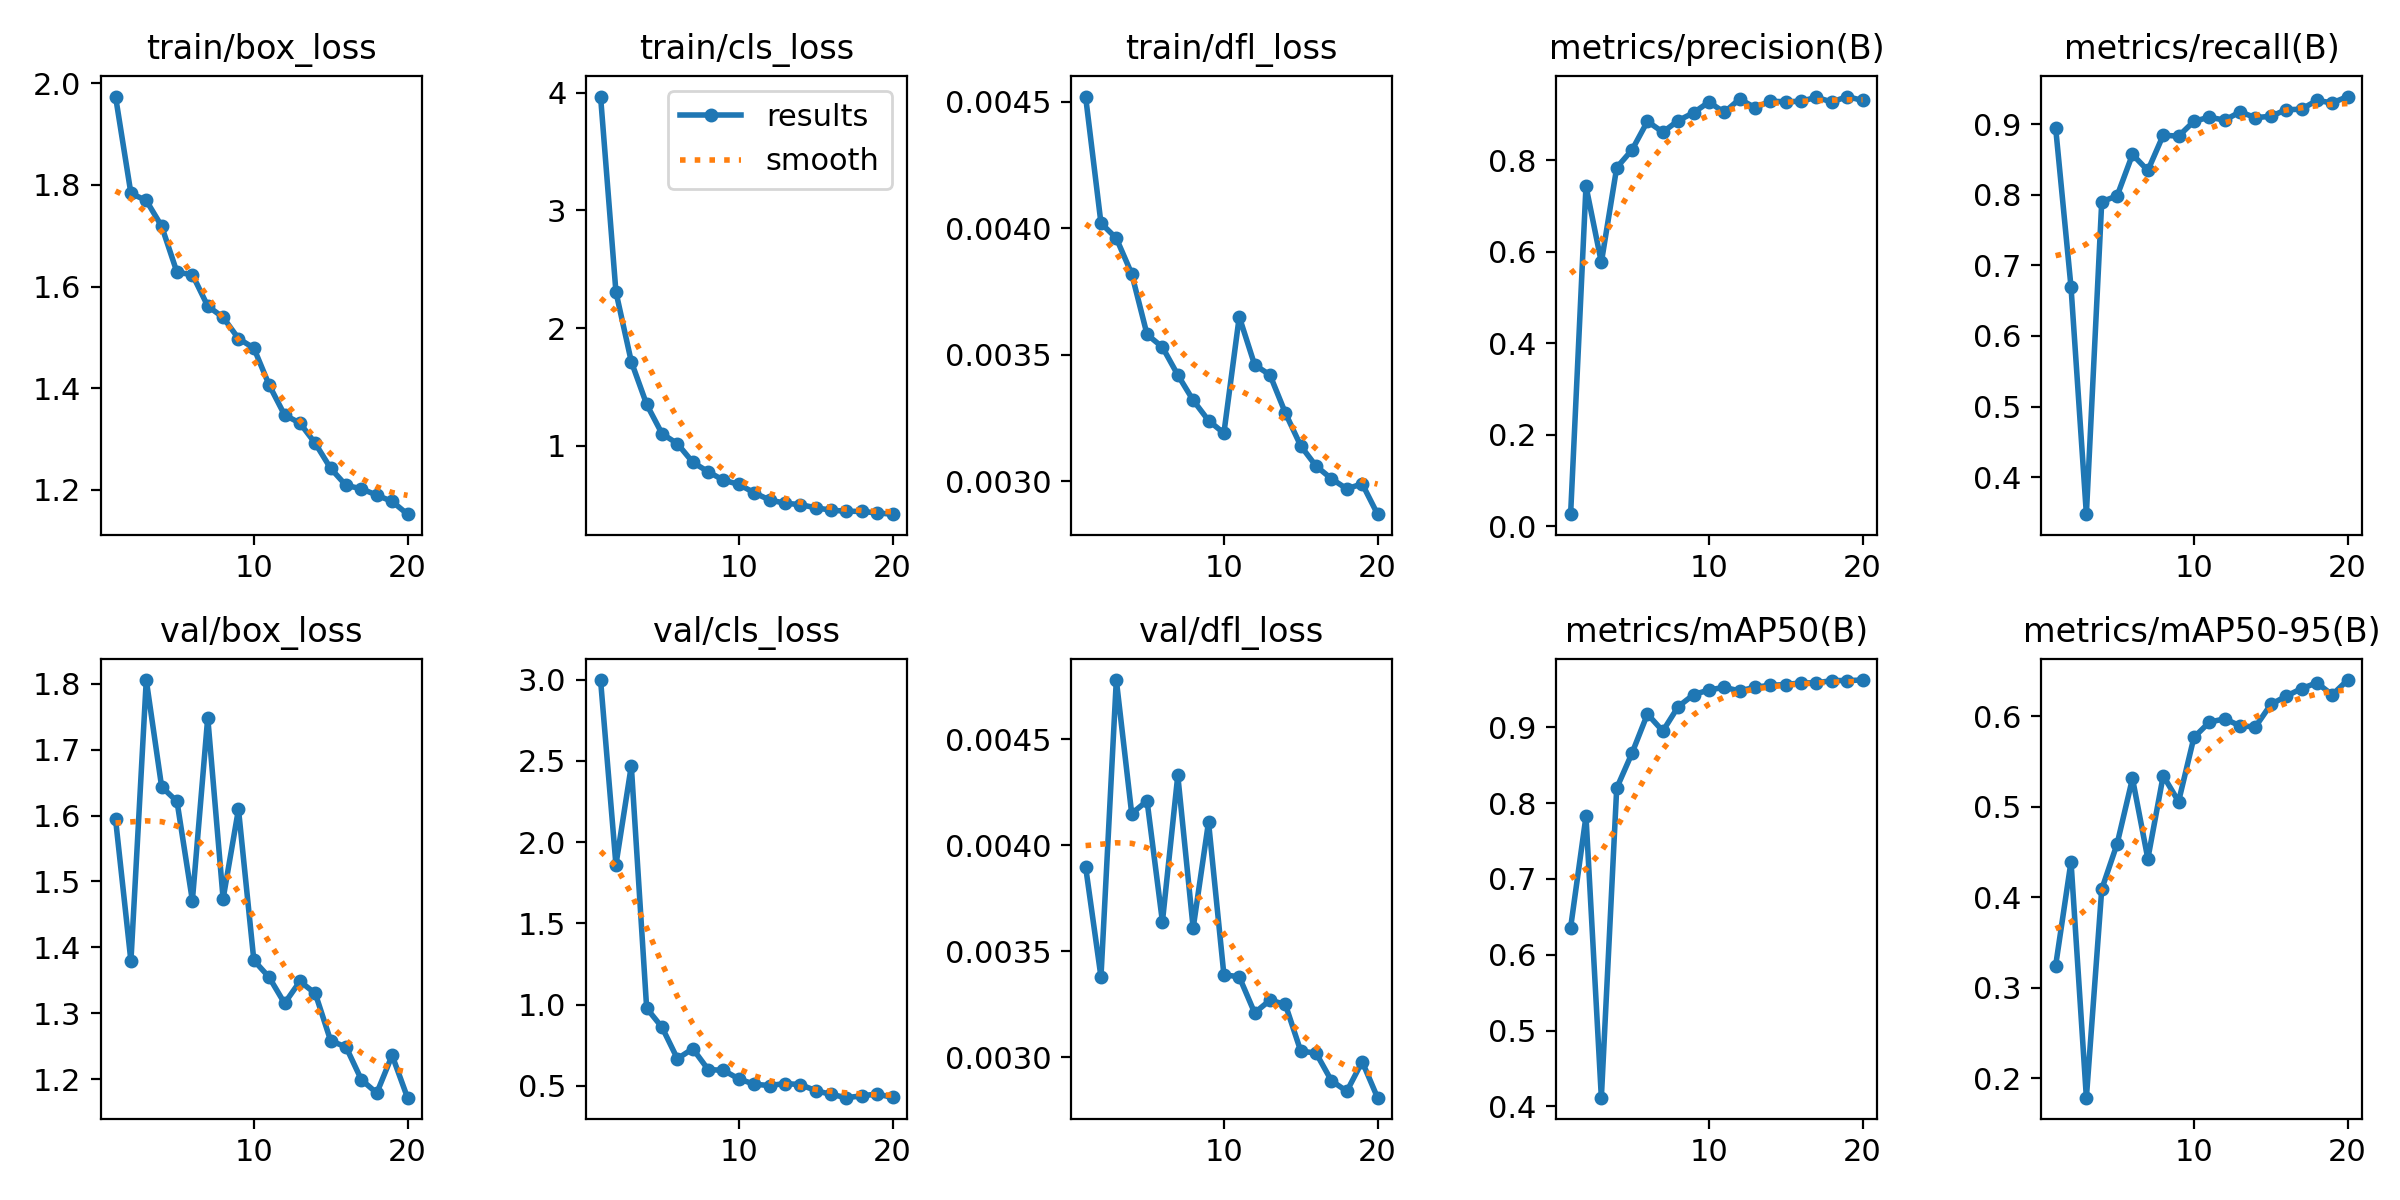
\includegraphics[width=0.8\textwidth]{robots-results}
  \caption{גרפי האימון של מודל זיהוי הרובוטים.}
\end{figure}

\begin{figure}[H] \centering
  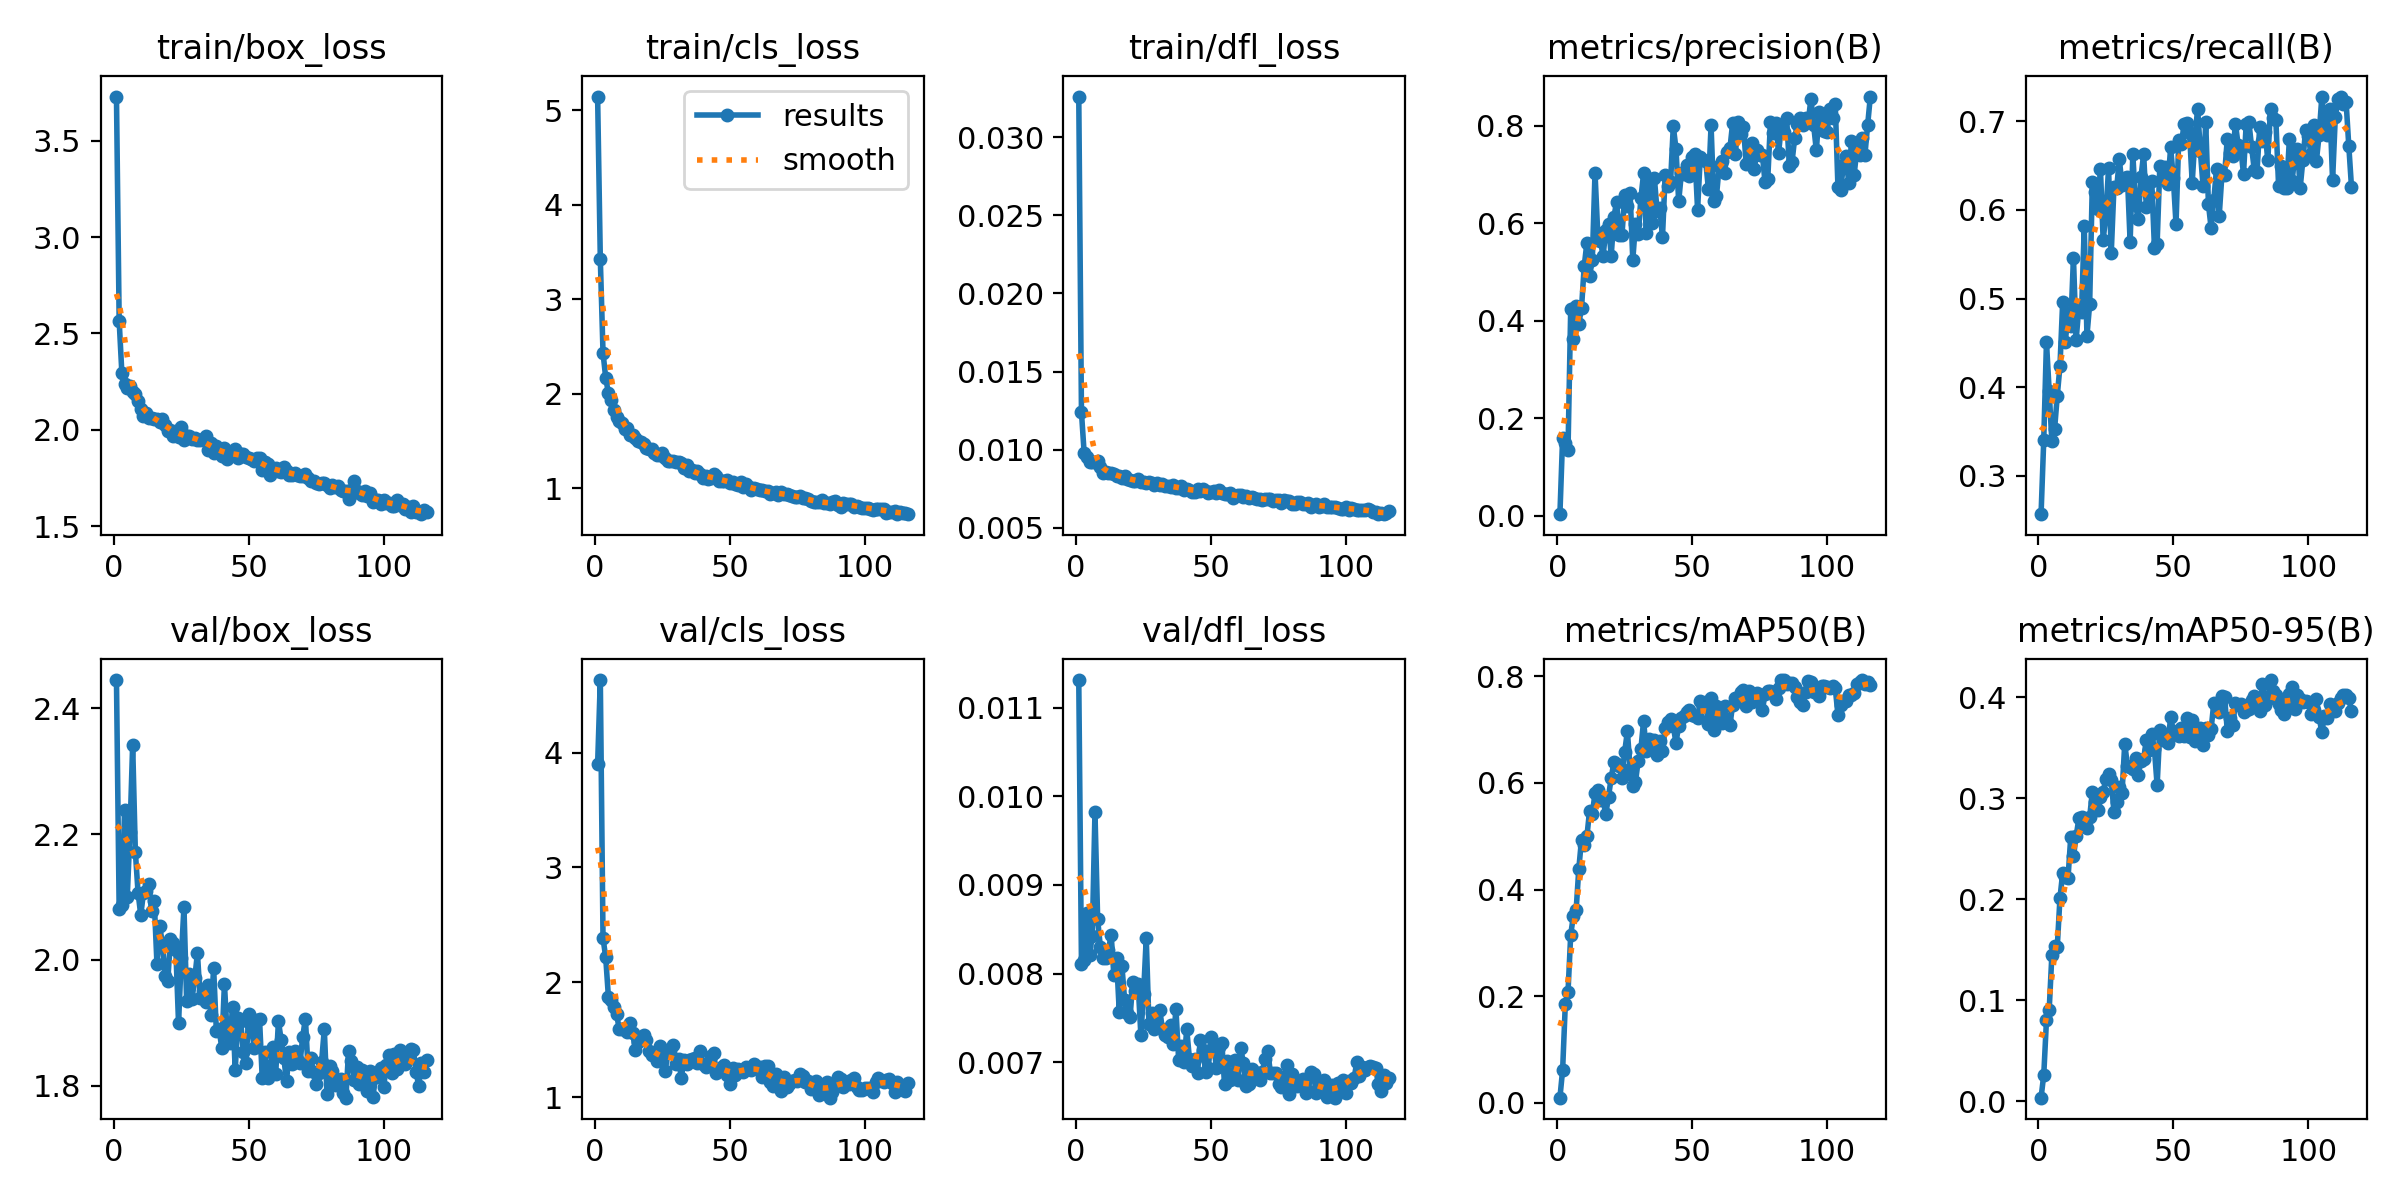
\includegraphics[width=0.8\textwidth]{digits-results}
  \caption{גרפי האימון של מודל זיהוי הספרות.}
\end{figure}

בטבלה הבאה מופיעות תוצאות האימון עבור כל אחד מהמודלים, שנמדדו על סט
הבדיקה שלא שימש לאימון או כוונון המודלים:

\begin{table}[H]
  \centering
  \begin{tabular}{|c|c|c|p{0.4\textwidth}|} \hline
    \textbf{מדד} & \textbf{מודל הרובוטים} & \textbf{מודל הספרות} & \textbf{משמעות המדד} \\ \hline
    Precision & 0.93 & 0.75 & מתוך כלל הזיהויים שהמודל החזיר, כמה היו נכונים. \\ \hline
    Recall & 0.94 & 0.78 & מתוך כלל האובייקטים האמיתיים, כמה המודל הצליח לזהות. \\ \hline
    mAP@50 & 0.97 & 0.85 & איכות הזיהוי כאשר חיזוי נחשב נכון אם החפיפה עם התיבה האמיתית היא לפחות 0.5 \textenglish{IoU}. \\ \hline
    mAP@50-95 & 0.66 & 0.43 & מדד מחמיר יותר שבודק איכות זיהוי בטווח ספי \textenglish{IoU} שונים. \\ \hline
  \end{tabular}
\end{table}

שני המודלים אומנו כמודלי \textenglish{YOLO} ולכן נמדדו באמצעות אותם
מדדי זיהוי אובייקטים. עם זאת, יש לפרש את המדדים בהקשר שונה: מודל
הרובוטים בוחן זיהוי של רובוטים וצבע ברית, ואילו מודל הספרות בוחן זיהוי
של ספרות קטנות על גבי רובוטים, משימה רגישה יותר לטשטוש, חסימות וזוויות
צילום.

מטריצות הבלבול (\textenglish{Confusion Matrix}) של המודלים ותוצאות
אימון מלאות לפי מחלקה מופיעות בנספח \ref{app:training}.

גרפי האימון, טבלת התוצאות ומטריצות הבלבול מצביעים על הבדל ברור בין שני
המודלים. מודל זיהוי הרובוטים יציב וחזק יותר, משום שההבחנה בין ברית
אדומה לכחולה מבוססת על סימן חזותי גדול וברור יחסית ברוב
הפריימים. לעומת זאת, מודל הספרות מתמודד עם משימה קשה יותר: הספרות
קטנות, מופיעות על באמפרים של רובוטים, ולעיתים מצולמות בזווית, בטשטוש
תנועה, בהסתרה חלקית או בתאורה לא אחידה. לכן גם כאשר מודל הספרות מצליח
לזהות ספרות רבות, יש יותר מקום לבלבול בין מחלקות, והמערכת אינה מסתמכת
על חיזוי מפריים יחיד אלא משלבת את תוצאות המודל לאורך זמן באמצעות
\textenglish{tracking}, צמצום לפי לוח המשחקים והצבעה מצטברת.

\subsection{ניסויים ושיפורים לאורך הדרך}

במהלך הפיתוח בוצעו כמה ניסויים ושינויים מהותיים. גם כאשר לא נשמרו כל
המספרים המדויקים של כל ריצה, אפשר לזהות בבירור את כיוון השיפור בכל שלב:

\begin{itemize}
\item \textbf{ניסוי 1 --- אימון ראשוני על נתונים נוחים וזיהוי בעיית
    \textenglish{Variance}:} בתחילת הדרך, חלק גדול מן הדוגמאות של
  הספרות הגיע ממקורות איכותיים יחסית. בשלב זה זיהיתי תופעה של
  \textenglish{High \newline Variance (Overfitting)}: המודל למד לזהות
  היטב את תמונות האימון והגיע לדיוק גבוה, אך כשהורץ על נתוני ולידציה
  המורכבים מסרטוני תחרות אמיתיים (עם טשטוש תנועה, חסימות ותאורה חלשה),
  הביצועים צנחו משמעותית. המודל למד להתאים את עצמו באופן הדוק מדי
  לתנאים האידיאליים ולא הצליח להכליל (\textenglish{Generalize}) את
  יכולת הזיהוי לתנאי אמת. העובדה שהמודל הגיע לביצועים גבוהים על נתוני
  האימון מעידה שלא סבלנו מבעיית \textenglish{High Bias
    (Underfitting)}.

\item \textbf{ניסוי 2 --- הוספת חיתוכים אוטומטיים כאמצעי
    \textenglish{Regularization}:} כדי לצמצם את הפער בין שגיאת האימון
  לשגיאת הוולידציה, נוספו למערך הנתונים דוגמאות שנחתכו אוטומטית מתוך
  סרטוני משחק. מערך הנתונים נעשה "מלוכלך" וריאלי יותר. הוספת רעש
  ויזואלי לנתוני האימון שימשה הלכה למעשה כסוג של רגולריזציה
  (\textenglish{Regularization}): היא מנעה מהמודל להסתמך רק על
  מאפיינים מושלמים, הכריחה אותו ללמוד מאפיינים עמידים
  (\textenglish{Robust Features}), וכך הקטינה את
  ה־\textenglish{Variance} ושיפרה את ההתאמה בין שלב האימון לזמן ההפעלה
  בפועל.
\item \textbf{ניסוי 3 --- כוונון אוגמנטציה:} אוגמנטציה מתונה מדי לא
  הספיקה כדי להתמודד עם זוויות קשות ותאורה משתנה, אך אוגמנטציה חזקה מדי
  גרמה לעיתים לפגיעה בקריאות הספרות. לכן נדרש איזון בין גיוון הנתונים
  לבין שמירה על צורת הספרה.
\item \textbf{ניסוי 4 --- פתרון מערכתי במקום שיפור מודל בלבד:} בשלב
  מסוים התברר שגם אם מודל הספרות לא מגיע לדיוק מושלם, עדיין אפשר לשפר
  משמעותית את המערכת כולה באמצעות שילוב התוצאה עם צבע הברית, לוח המקצים
  והצבעה מצטברת לאורך זמן. זהו שינוי חשוב בגישת הפיתוח: מעבר משיפור
  מודל בודד לשיפור מערכת מלאה.
\end{itemize}

\subsection{אתגרים מרכזיים ופתרונות}

תהליך האימון חשף כמה אתגרים מרכזיים:

\begin{itemize}
\item \textbf{פער בין נתוני אימון לנתוני אמת:} תמונות נקיות או חיתוכים
  ידניים לא תמיד מייצגות נאמנה את סרטוני התחרות. הפתרון היה להוסיף יותר
  דוגמאות מתוך צינור העבודה האמיתי.
\item \textbf{אובייקטים קטנים ודומים:} הספרות קטנות, וחלקן דומות זו
  לזו במיוחד כאשר יש טשטוש תנועה. הפתרון היה גם הרחבת הנתונים וגם
  הסתמכות על לוגיקת החלטה מערכתית לאחר האימון.
\item \textbf{סיכון ל־\textenglish{Overfitting}:} במיוחד במודל הספרות,
  גודל מערך הנתונים היה מוגבל יחסית. שימוש באוגמנטציה ובדוגמאות מגוונות
  יותר צמצם את הבעיה.
\item \textbf{מגבלת משאבים:} סביבת \textenglish{Colab} נוחה לאימון,
  אך עדיין דורשת תכנון זהיר של מספר הניסויים ושל זמני הריצה. לכן חלק מן
  האיטרציות בוצעו תחילה על קבוצות נתונים קטנות יותר או עם בדיקות מהירות
  לפני ריצות מלאות.
\end{itemize}

\subsection{זמן אימון וחומרה}

כל ריצות האימון בוצעו על גבי \textenglish{GPU} מסוג
\textenglish{NVIDIA T4} ב־\textenglish{Google Colab}.

\begin{itemize}
\item \textbf{זמן אימון סופי של מודל הרובוטים:} \textbf{20.59 דקות}.
\item \textbf{זמן אימון סופי של מודל הספרות:} \textbf{10.92 דקות}.
\item \textbf{מספר ריצות ניסוי כולל:} \textbf{כ־8--10}.
\end{itemize}

גם ללא המספרים המדויקים, חשוב לציין שהחלק הארוך באמת בפרויקט לא היה רק
זמן האימון עצמו, אלא זמן האיסוף, התיוג והשיפור האיטרטיבי של הנתונים.
במובן זה, הפרויקט היה \textbf{Data-Centric} לא פחות משהיה
\textbf{Model-Centric}.

\subsection{סיכום תהליך האימון}

תהליך האימון הוביל לשתי מסקנות עיקריות. ראשית, מודל זיהוי הרובוטים היה
חזק יחסית כבר בשלבים מוקדמים והגיע במהירות לביצועים מספקים. שנית,
האתגר האמיתי בפרויקט היה מודל זיהוי הספרות, שבו איכות הנתונים והריאליזם
של הדוגמאות היו קריטיים לא פחות מהארכיטקטורה עצמה.

לכן, ההצלחה של המערכת אינה נובעת רק מבחירת מודל טוב, אלא משילוב בין
אימון סביר של שני מודלים, שיפור מתמיד של מערך הנתונים, ושכבת החלטה
נוספת שמנצלת את הפלטים של המודלים בצורה חכמה. זהו בדיוק המעבר מפרויקט
של "אימון רשת" לפרויקט של הנדסת מערכת מבוססת למידת מכונה.

\section{השוואת ביצועים}
\subsection{בחירת ה־\textenglish{Baseline}}

בפרויקט כמו \textenglish{AutoScout}, שבו ההחלטה הסופית מתקבלת מצינור
רב־שלבי, ה־\textenglish{Baseline} המתאים הוא גרסה פשוטה יותר של אותו
צינור ולאו דווקא מודל חלופי. מטרת ההשוואה היא לבדוק מה כל שכבה מוסיפה:
צמצום מועמדים לפי המקצה, צבע ברית, זיהוי ספרות, מעקב וצבירת ראיות
לאורך זמן.

\subsection{קווי הבסיס שנבחרו}

להערכת המערכת ובידוד התרומה של כל שכבת לוגיקה, הוגדרו שני סוגים שונים
של קווי בסיס:

\paragraph{קווי בסיס תיאורטיים-הסתברותייים:}
קווי בסיס אלו מייצגים מערכת ``עיוורת'' לחלוטין ומגדירים את רצפת
הביצועים הסטטיסטית התיאורטית של הבעיה:

\begin{itemize}
\item \textbf{ניחוש אקראי מתוך שש קבוצות:} מאחר שבכל מקצה משתתפות שש
  קבוצות בלבד, מערכת שאין לה מידע נוסף יכולה רק לנחש. הדיוק הצפוי הוא
  \textbf{\(1/6\)}, כלומר כ־\textbf{0.17}.
  
\item \textbf{ניחוש מתוך הברית הנכונה בלבד:} אם ידוע רק צבע הברית,
  מרחב החיפוש מצטמצם לשלוש קבוצות. במקרה כזה הדיוק הצפוי הוא
  \textbf{\(1/3\)}, כלומר כ־\textbf{0.33}.
\end{itemize}

\paragraph{קו בסיס אלגוריתמי־אמפירי:}

\begin{itemize}
\item \textbf{זיהוי ספרות נקודתי ללא צבירה לאורך זמן:} קו בסיס זה
  משתמש בזיהוי הספרות שעל הבאמפר ומשווה אותן לקבוצות האפשריות, אך מקבל
  החלטה על סמך פריים בודד. הוא טוב יותר מניחוש, אבל רגיש לטשטוש תנועה,
  לחסימות ולזיהוי חלקי. קו בסיס זה נמדד אמפירית על נתוני האמת, ומטרתו
  להוכיח את נחיצותה של שכבת קבלת ההחלטות במערכתית שפיתחתי.
\end{itemize}

\subsection{ניתוח ההשוואה}

מאחר שקווי הבסיס התיאורטיים מייצגים גבולות הסתברותיים מתמטיים ולא
מערכות תוכנה שרצו בפועל, הטבלה שלהלן מפרידה בין המדדים התיאורטיים לבין
תוצאות הניסוי האמפירי.

הניסוי האמפירי בוצע באמצעות תהליך תיקוף ידני מבוסס דגימה, על מקצי
תחרות מלאים, כאשר בשל אילוצי תיוג ידני, קו הבסיס האלגוריתמי נמדד על
תת־קבוצה מייצגת של שני מקצים:

\begin{table}[H]
  \centering
  \begin{tabular}{|>{\raggedleft\arraybackslash}p{0.125\textwidth}|>{\raggedleft\arraybackslash}p{0.125\textwidth}|>{\raggedleft\arraybackslash}p{0.125\textwidth}|>{\raggedleft\arraybackslash}p{0.125\textwidth}|>{\raggedleft\arraybackslash}p{0.125\textwidth}|>{\raggedleft\arraybackslash}p{0.125\textwidth}|>{\raggedleft\arraybackslash}p{0.125\textwidth}|}
    \hline
    \textbf{שיטה} & \textbf{סוג המדד} & \textbf{מספר מקצים שנמדדו} & \textbf{סך מופעי רובוט} & \textbf{סך שיוכים נכונים} & \textbf{תוצאה} \\ \hline
    ניחוש אקראי & תיאורטי & -- & -- & -- & \textbf{0.17} \\ \hline
    ניחוש לפי ברית & תיאורטי & -- & -- & -- & \textbf{0.33} \\ \hline
    זיהוי ספרות ללא צבירה & אמפירי & 2 & 183 & 102 & \textbf{0.56} \\ \hline
    המערכת המלאה & אמפירי & 3 & 273 & 204 & \textbf{0.75} \\ \hline
  \end{tabular}
  \caption{השוואת קווי בסיס למערכת המלאה.}
  \label{tab:baseline_comparison}
\end{table}

ההשוואה מראה שכל רכיב מוסיף סוג אחר של מידע:
 
\begin{itemize}
\item \textbf{מספר המקצה} מצמצם מיד את מרחב החיפוש לשש קבוצות בלבד.
\item \textbf{צבע הברית} מצמצם אותו עוד יותר לשלוש מועמדות אפשריות.
\item \textbf{זיהוי הספרות} מוסיף רמז זהותי חזק, אך הוא רועש כאשר הבאמפר
  מוסתר, מטושטש או מצולם בזווית קשה.
\item \textbf{המעקב וההצבעה המצטברת} מאפשרים לצבור ראיות לאורך זמן,
  ולכן מפחיתים את ההשפעה של טעויות מקומיות בפריימים בודדים.
\end{itemize}

מכאן שהיתרון של המערכת המלאה אינו נובע רק ממודל ספרות טוב יותר, אלא
מכך שהיא פותרת את הבעיה ברמת \textbf{עקבה שלמה} ולא ברמת פריים יחיד.

\subsection{השוואה לפתרונות קיימים}

אפשר להשוות את הפרויקט גם לשתי משפחות נפוצות של פתרונות:

\begin{itemize}
\item \textbf{סקאוטינג ידני:} גמיש ועתיר הקשר אנושי, אך דורש כוח אדם רב,
  אינו שומר מסלולים מלאים, ורגיש לעייפות ולטעויות הקלדה.

\item \textbf{מערכות \textenglish{Detection + Tracking} כלליות:} מסוגלות
  לזהות ולעקוב אחר רובוטים, אך ללא ידע דומייני נוסף הן אינן פותרות היטב
  את שאלת הזהות של כל רובוט כאשר כמה רובוטים דומים מופיעים יחד על
  המגרש.
\end{itemize}

היתרון של \textenglish{AutoScout} הוא בשילוב בין אוטומציה לבין ידע
דומייני: מצד אחד המערכת מהירה ועקבית יותר מסקאוטינג ידני, ומצד שני היא
מנצלת את לוח המשחקים של המקצה --- מידע שמערכות מעקב כלליות אינן מנצלות.

\subsection{מסקנה מן ההשוואה}

המסקנה המרכזית היא שהפתרון החזק ביותר לבעיה זו אינו מודל יחיד, אלא
מערכת שמחברת זיהוי, מעקב וידע מוקדם. זו גם הנקודה שבה \textenglish{AutoScout}
שונה מקווי בסיס פשוטים יותר ומכלי מעקב כלליים.

\section{תוצאות והדגמות}
\subsection{תוצאות כמותיות}

הערכת המערכת בוצעה בכמה רמות: זיהוי הרובוטים, זיהוי הספרות, והשיוך
הסופי של עקבה לקבוצה.

כדי להעריך את ביצועי המערכת המלאה מקצה לקצה, בוצע ניסוי אמפירי המבוסס
על מתודולוגיית תיקוף ידני. במסגרת הבדיקה נדגמו מופעי רובוטים במרווחי
זמן קבועים מתוך שלושה מקצי תחרות מלאים משלוש תחרויות שונות, כדי לייצר
``\textenglish{Ground Truth}'' להשוואה. ``מופע רובוט'' הוגדר כרגע שבו
רובוט נראה על המסך במידה שמאפשרת לאדם לעקוב אחריו לאורך הסרטון, גם אם
מספר הקבוצה אינו קריא באותו פריים ספציפי. מופע נספר כהצלחה רק אם
המערכת שייכה באותו רגע את העקבה לקבוצה הנכונה.

מדד הדיוק המערכתי מוגדר כיחס בין מספר המופעים שבהם המערכת שייכה
בהצלחה את הרובוט לקבוצה הנכונה לבין סך המופעים הכולל שנדגם. בניסוי זה
נדגמו בסך הכל 273 מופעי רובוט לאורך שלושת המקצים. המערכת זיהתה ושייכה
בהצלחה ובאופן מדויק את הרובוט לקבוצתו ב־204 מופעים, נתון המוביל למדד
דיוק מערכתי של $\frac{204}{273} \approx 0.75$.

\begin{table}[H]
  \centering
  \begin{tabular}{|c|c|c|c|c|}
    \hline
    \textbf{מקצה} &
    \textbf{מופעי רובוט שנדגמו} &
    \textbf{שיוכים נכונים} &
    \textbf{שיוכים חסרים או שגויים} &
    \textbf{דיוק שיוך} \\ \hline

    1 & 91 & 71 & 20 & 78.0\% \\ \hline
    2 & 88 & 61 & 27 & 69.3\% \\ \hline
    3 & 94 & 72 & 22 & 76.6\% \\ \hline
    \textbf{סה''כ} & \textbf{273} & \textbf{204} & \textbf{69} & \textbf{74.7\%} \\ \hline
  \end{tabular}
  \caption{דיוק השיוך המערכתי לפי מקצה.}
\end{table}

בטבלה זו לא בוצעה הפרדה כמותית בין סוגי הכשל. כלומר, מופע שלא נספר
כהצלחה יכול לנבוע מזיהוי רובוט חסר, איבוד עקבה, היעדר שיוך, או שיוך
לקבוצה שגויה. שגיאות אלו מפורטות בהמשך הפרק. מטרת המדד היא למדוד את
הצלחת המערכת מקצה לקצה, ולא לבודד את מקור השגיאה בכל רכיב בנפרד. בגרסה
עתידית ניתן לבצע ניתוח שגיאות מפורט יותר שיחלק את הכשלים לקטגוריות
כגון זיהוי רובוטים, מעקב, זיהוי ספרות ושיוך סופי.

משמעותו הפרקטית של נתון זה היא שבמדגם שנבדק, מתוך שישה רובוטים
הנמצאים בדרך כלל על המגרש, המערכת מצליחה לשייך נכון בממוצע כארבעה עד
חמישה רובוטים במצבים שבהם הם נראים על המסך וניתנים למעקב אנושי.

\begin{table}[H]
  \centering
  \begin{tabular}{|c|c|c|}
    \hline
    \textbf{רכיב} & \textbf{מדד} & \textbf{תוצאה} \\ \hline
    מודל זיהוי הרובוטים & \textenglish{mAP@50} & \textbf{0.97} \\ \hline
    מודל זיהוי הספרות &\textenglish{Precision}  ברמת הספרה & \textbf{0.75} \\ \hline
    שיוך סופי של עקבה לקבוצה & דיוק זיהוי ושיוך מתוך סרטון & \textbf{0.75} \\ \hline
    ביצועי הרצה & \textenglish{FPS} & \textbf{30--60} \\ \hline
  \end{tabular}
  \caption{סיכום התוצאות הכמותיות של המערכת.}
\end{table}

בנוסף למדדי הדיוק, המערכת מצליחה לייצר עבור כל קבוצה מסלול תנועה רציף
ומוחלק שאותו אפשר להציג לאחר המקצה לצורך ניתוח משחק.

מהתוצאות עולה שזיהוי הרובוטים הוא הרכיב היציב יותר, בעוד שזיהוי הספרות
הוא עדיין צוואר הבקבוק של המערכת. למרות זאת, השילוב של זיהויי ספרות
מצטברים לאורך זמן עם צבע הברית ורשימת הקבוצות האפשריות, מאפשר למערכת
להגיע לדיוק סופי גבוה משמעותית מזה שהיה מתאפשר מזיהוי ספרות בלבד.

\subsection{דוגמאות הצלחה}

בבדיקות המערכת נצפו כמה דפוסי הצלחה ברורים:

\begin{itemize}
\item \textbf{זיהוי ותחימה יציבים של ששת הרובוטים:} כאשר הרובוטים
  מרוחקים יחסית זה מזה ואינם חוסמים זה את זה, מודל הזיהוי והמעקב
  מצליחים לשמור על עקבות נקיות ויציבות לאורך זמן.

\item \textbf{התאוששות משגיאת ספרות בודדת:} גם כאשר פריים אחד מחזיר
  זיהוי חלקי או שגוי של הספרות, מנגנון ההצבעה המצטבר מונע מן המערכת
  לקפוץ מיד לזהות שגויה. לאחר כמה פריימים טובים יותר, המערכת מתכנסת
  שוב לקבוצה הנכונה.

\item \textbf{שיוך זהות נכון בזכות שילוב כמה רמזים:} במקרים רבים,
  הספרות לבדן אינן מספיקות. עם זאת, כאשר הן משולבות עם צבע הברית ועם
  רשימת שש הקבוצות האפשריות במקצה, אפשר להגיע לזהות נכונה גם אם רק חלק
  מן הספרות נקראו היטב.

\item \textbf{הפקת מסלולים שימושיים לניתוח:} גם במקרים שבהם היו חסרים
  פריימים בודדים או זיהויים לא מושלמים, האינטרפולציה וההחלקה הצליחו
  להפיק מסלול תנועה סביר, קריא ורציף לשימוש בתצוגת
  ה־\textenglish{Replay}.
\end{itemize}

דוגמאות וויזואליות להצלחות של זיהויי רובוטים וזיהויי ספרות מצורפות בנספח \ref{app:success} באיור \ref{fig:success}.

\subsection{דוגמאות כישלון וניתוח טעויות}

לצד ההצלחות, המערכת עדיין נכשלת בכמה סוגי מצבים שחוזרים על עצמם:

\paragraph{כשלים חזותיים:} הכשלים הבאים נובעים ממגבלות המידע החזותי
הזמין למודלים.

\begin{tabular}{|p{0.3\textwidth}|r|p{0.4\textwidth}|} \hline 
  \textbf{תמונה} & \textbf{סוג הכשל} & \textbf{השפעה על המערכת} \\ \hline
  \begin{minipage}[t]{\linewidth}
    \vspace{0pt}
    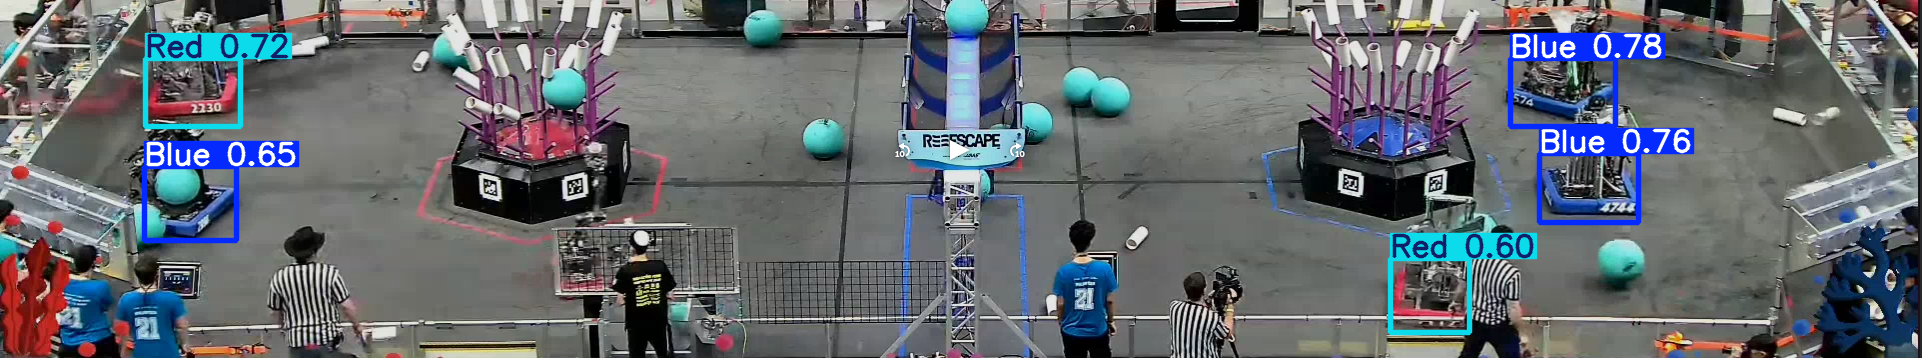
\includegraphics[width=\linewidth]{robots-failure-occluded}
    \vspace{0pt}
  \end{minipage}  & חסימת באמפר & הספרות או הרובוט כולו אינם נראים למשך זמן ממושך ולכן קשה לצבור ראיות מספיקות לזיהוי הקבוצה \\ \hline
  \begin{minipage}[t]{\linewidth}
    \vspace{0pt}
    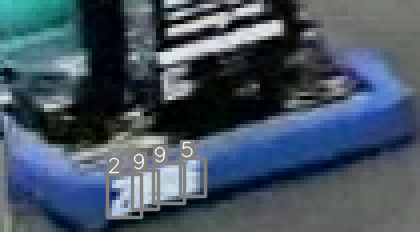
\includegraphics[width=\linewidth]{digits-failure-blur}
    \vspace{0pt}
  \end{minipage} & טשטוש תנועה & זיהוי הספרות מחזיר לעיתים תוצאה חלקית או שגויה \\ \hline
  \begin{minipage}[t]{\linewidth}
    \vspace{0pt}
    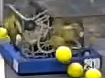
\includegraphics[width=\linewidth]{digits-failure-gp}
    \vspace{0pt}
  \end{minipage} & שונות בין עונות & ביצועי המודלים עלולים לרדת כשהם
  מופעלים על עונה שלא הופיעה בנתוני האימון, בשל ההבדלים הגדולים במבנה
  הרובוטים, במגרש ובחפצי המשחק \\ \hline
\end{tabular}

\paragraph{כשלים מערכתיים:} הכשלים הבאים נובעים מההתנהגות וקבלת
ההחלטות של המערכת לאורך זמן.

\begin{tabular}{|p{0.15\textwidth}|p{0.4\textwidth}|p{0.3\textwidth}|} \hline
  \textbf{סוג הכשל} & \textbf{השפעה על המערכת} & \textbf{מנגנון התמודדות קיים} \\ \hline
  מספרי קבוצות דומים & עלול להיווצר בלבול בין שתי קבוצות מועמדות & דרישת מרווח מינימלי בין שתיהן \\ \hline
  החלפת \textenglish{Track IDs} & שיוך של רובוטים עלול להיפגע אחרי הצטלבות מסלולים או הסתרה ממושכת & איפוס השיוך וצבירת ראיות מחדש \\ \hline
\end{tabular}

דוגמאות הכישלון חשובות לא פחות מן ההצלחות, משום שהן מראות היכן המערכת
עדיין פגיעה ואילו שיפורים עתידיים יהיו בעלי התרומה הגדולה ביותר.

\subsection{מדריך למשתמש: תהליך השימוש והדגמת המערכת}

השימוש באפליקציית \textenglish{AutoScout} מתבצע בשלושה מסכים עיקריים:
מסך העלאת הסרטון, מסך התקדמות העיבוד, ומסך הצפייה בתוצאות.
מדריך זה מתאר את הפעולות שהמשתמש מבצע בכל אחד מהמסכים.

\subsubsection{מסך העלאת סרטון}

במסך הראשון מזינים את מספר המקצה ובוחרים את קובץ הווידאו שרוצים לנתח.
תחילה ממלאים את השדה \textenglish{Match Number}, ולאחר מכן לוחצים על
\textenglish{Select Video} כדי לבחור את הסרטון מהמחשב.

לאחר שנבחר קובץ וידאו, לוחצים על \textenglish{Upload} כדי לשלוח את הסרטון
לעיבוד. אם לא נבחר סרטון, כפתור ההעלאה אינו פעיל.

\begin{figure}[H]
  \centering
  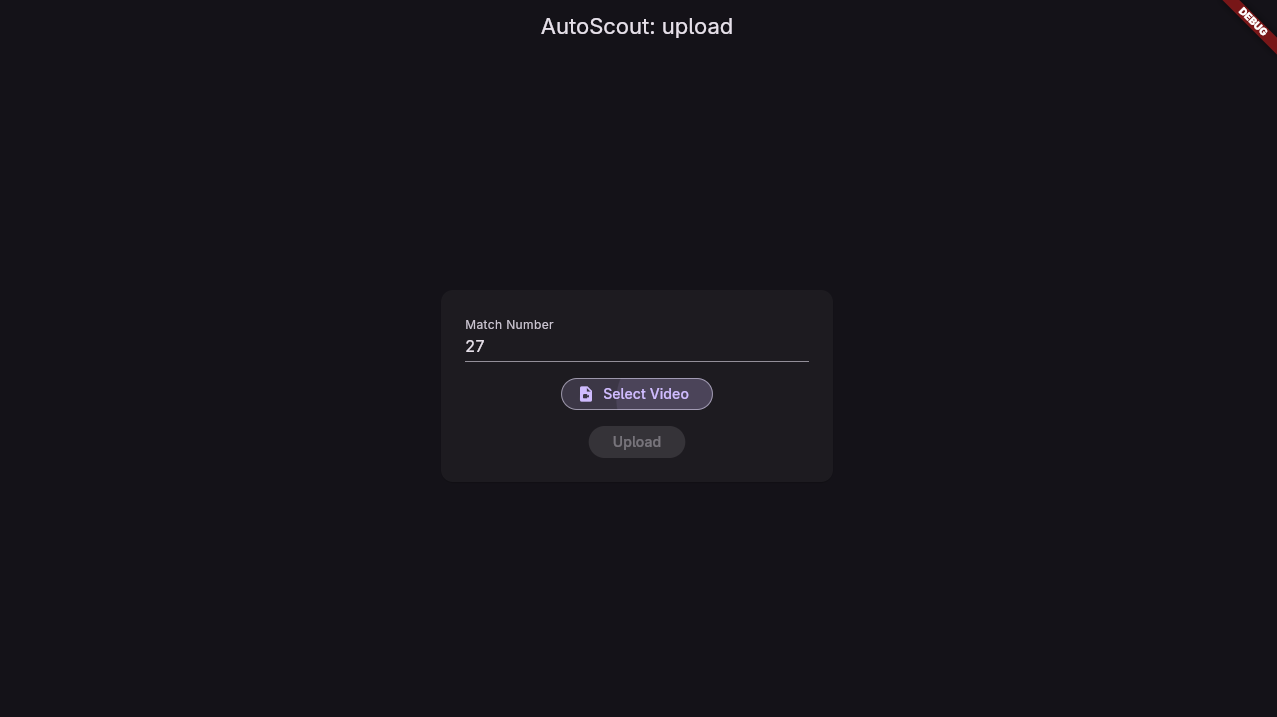
\includegraphics[width=0.95\textwidth]{app-upload.png}
  \caption{מסך העלאת הסרטון והזנת מספר המקצה.}
\end{figure}

\subsubsection{מסך התקדמות העיבוד}

לאחר העלאת הסרטון מופיע מסך התקדמות העיבוד.
במסך זה ניתן לראות את מצב הניתוח של הסרטון בזמן שהשרת מעבד אותו.

המסך מציג את מספר הפריים הנוכחי מתוך כלל הפריימים, את קצב העיבוד
בפריימים לשנייה, ואת זמן הסיום המשוער. בנוסף מוצג פס התקדמות המאפשר
לעקוב אחר קצב ההתקדמות של הניתוח.

מסך זה נועד להראות שהמערכת עדיין עובדת ושאין צורך להעלות את הסרטון מחדש
בזמן שהעיבוד מתבצע.

\begin{figure}[H]
  \centering
  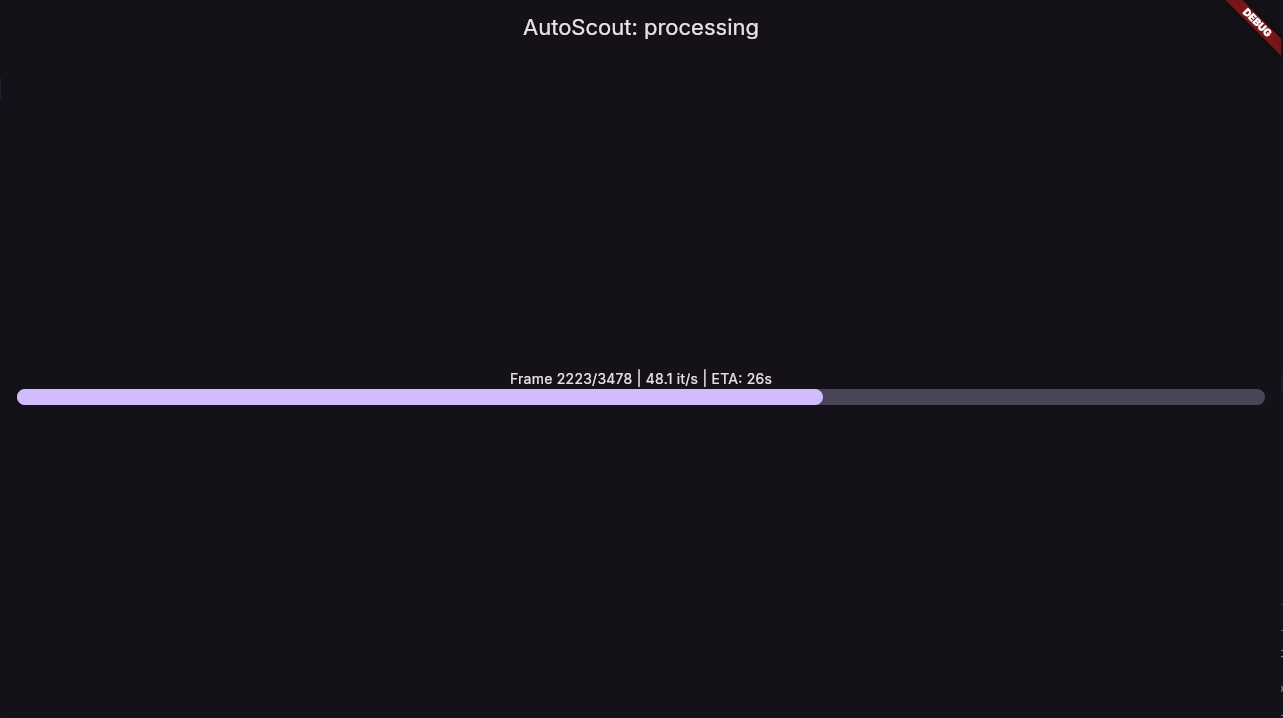
\includegraphics[width=0.95\textwidth]{app-progress.png}
  \caption{מסך התקדמות העיבוד של הסרטון.}
\end{figure}

\subsubsection{מסך צפייה בתוצאות}

לאחר סיום העיבוד מופיע מסך התוצאות.
במסך זה מוצג הסרטון לאחר הניתוח, יחד עם תוצאות המעקב והשיוך שהמערכת
הפיקה עבור הרובוטים.

במסך זה ניתן:
\begin{itemize}
    \item להפעיל ולעצור את הסרטון באמצעות כפתור הניגון.
    \item לעבור לנקודות זמן שונות במקצה באמצעות פס הזמן.
    \item לצפות בסימונים ובמספרי הקבוצות שהמערכת מציגה על גבי הסרטון.
    \item להשתמש בכפתור העליון כדי להציג או להסתיר את הסרטון המקורי מאחורי תוצאות המעקב.
    \item לחזור למסך הקודם באמצעות כפתור החזרה.
\end{itemize}

מסך זה מאפשר לבדוק את תוצאת המערכת בצורה חזותית. במקום להציג רק טבלה או
קובץ פלט, ניתן לראות את תוצאות המעקב והשייכות ישירות על גבי הסרטון.

\begin{figure}[H]
  \centering
  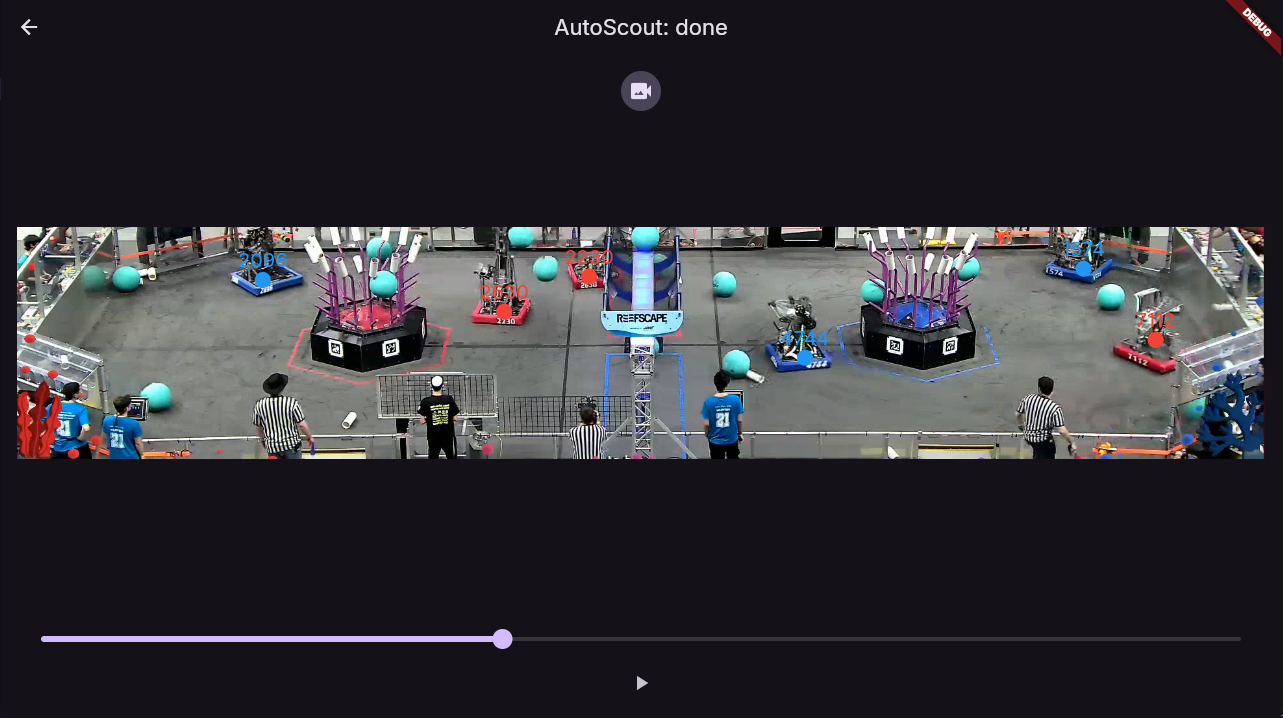
\includegraphics[width=0.95\textwidth]{app-replay.png}
  \caption{מסך צפייה בתוצאות לאחר סיום הניתוח.}
\end{figure}

\subsubsection{סיכום תהליך השימוש}

תהליך השימוש המלא במערכת הוא:
\begin{enumerate}
    \item מזינים מספר מקצה.
    \item בוחרים קובץ וידאו.
    \item לוחצים על \textenglish{Upload}.
    \item ממתינים לסיום העיבוד במסך ההתקדמות.
    \item צופים בתוצאות במסך הצפייה.
\end{enumerate}

\href{https://www.youtube.com/watch?v=x60OrcgcYnA}{\textenglish{AutoScout}: הדגמה} --- קישור לסרטון הדגמה קצר של המערכת בפעולה.

\subsection{סיכום פרק התוצאות}

התוצאות מראות שהמערכת חזקה בזיהוי הרובוטים, ושימושית גם בשיוך קבוצות
למרות חולשות קיימות בזיהוי הספרות.

\section{דיון ומסקנות}
\subsection{ניתוח התוצאות}

מן התוצאות עולה שזיהוי הרובוטים הוא רכיב חזק ויציב, ואילו זיהוי
הספרות הוא עדיין החלק הרגיש יותר. למרות זאת, המערכת כולה נשארת שימושית
מפני שההחלטה הסופית אינה נשענת על מקור מידע יחיד אלא על צבירת ראיות
לאורך זמן.

\subsection{מגבלות ומקרי קצה}

למרות ההישגים, למערכת עדיין יש כמה מגבלות ברורות:

\begin{itemize}
\item \textbf{תלות באיכות הצילום:} סרטונים מטושטשים, רחוקים מדי או
  כאלה שצולמו בזווית לא נוחה מקשים מאוד על קריאת הספרות ועל שמירת
  המעקב.

\item \textbf{חסימות בין רובוטים:} כאשר כמה רובוטים נצמדים או חוצים זה
  את זה, יש סיכון לאיבוד עקבות או להחלפת זהויות זמנית.

\item \textbf{היעדר \textenglish{Re-Identification} חזותי מלא:} המערכת
  הנוכחית אינה לומדת חתימה חזותית עמוקה של כל רובוט. לכן, לאחר חסימה
  ארוכה, היא מסתמכת בעיקר על הזיהוי מחדש של הספרות ועל לוגיקת ההצבעה.

\item \textbf{הערכת ביצועים חלקית:} חלק מן המדדים במערכת המלאה עדיין
  דורשים הערכה כמותית מסודרת יותר, למשל דיוק שיוך סופי על קבוצת בדיקה
  ייעודית או מדדי מעקב פורמליים.
\end{itemize}

מגבלות אלו אינן מבטלות את השימושיות של המערכת, אך הן מגדירות היטב את
גבולות היכולת הנוכחיים שלה.

דוגמאות וויזואליות לכישלונות של המודלים מצורפות בנספח \ref{app:success_failure} באיור \ref{fig:failure}.

\subsection{מיקום ביחס למצב הקיים}

הפרויקט אינו מתיימר להתחרות ישירות ב־\textenglish{state of the art}
האקדמי בזיהוי אובייקטים, במעקב או ב־\textenglish{OCR}. במקום זאת, הוא
מכוון לבעיה יישומית, ממוקדת ומוגדרת היטב: סקאוטינג אוטומטי של משחקי
\textenglish{FRC} מתוך סרטון וידאו מהיציע.

בהקשר זה, התרומה של הפרויקט היא בעיקר הנדסית ומערכתית:

\begin{itemize}
\item שילוב של שני מודלי זיהוי שונים בתוך צינור עיבוד אחד.
\item ניצול ידע דומייני חזק מאוד מן הלו"ז של המקצה.
\item המרה של פלטי ראייה ממוחשבת למסלולי תנועה ולייצוג שימושי לסקאוטינג.
\item חיבור בין צד שרת, ממשק משתמש ואלגוריתם ניתוח בפלטפורמה אחת.
\end{itemize}

לכן, הערך של המערכת נמדד פחות בשאלה האם היא שוברת שיאי דיוק כלליים,
ויותר בשאלה האם היא פותרת בפועל בעיה אמיתית בעולם ה־\textenglish{FRC}.

\subsection{הצעות לשיפור עתידי}

אם היו לי עוד כמה חודשי פיתוח, יש כמה כיוונים שהייתי שמח להמשיך בהם:

\begin{itemize}
\item \textbf{איסוף מערך נתונים גדול וריאלי יותר:} במיוחד עבור ספרות
  בתנאי צילום קשים, כדי לשפר את ההכללה של מודל הספרות.

\item \textbf{הוספת רכיב \textenglish{Re-Identification}:} מודל חזותי
  נוסף שיוכל לסייע בשמירת זהות גם כאשר הספרות אינן נראות לאורך זמן.

\item \textbf{כיול גאומטרי של המגרש:} התאמת נקודות התמונה לקואורדינטות
  אמיתיות על המגרש, כך שהמסלולים ימדדו ביחידות מרחק אמיתיות ולא רק
  במרחב הפיקסלים.

\item \textbf{פרוטוקול הערכה מסודר יותר:} יצירת סט בדיקה מסומן היטב עם
  אמת מידה מלאה לשיוך קבוצות ולעקיבה, כדי לאפשר השוואה כמותית חזקה יותר
  בין גרסאות שונות של המערכת.

\item \textbf{אופטימיזציה לביצועים:} צמצום זמן הריצה ושיפור היכולת
  לעבוד קרוב יותר לזמן אמת גם על חומרה חלשה יותר.
\end{itemize}

\subsection{שיקולים אתיים ושימוש אחראי}

מבחינה אתית, זהו פרויקט בעל סיכון נמוך יחסית, משום שהוא מנתח משחקי
רובוטיקה ציבוריים ולא מידע רפואי, פיננסי או אישי רגיש. עם זאת, עדיין יש
כמה שיקולים חשובים:

\begin{itemize}
\item \textbf{אמינות ההחלטות:} אם המערכת טועה בזיהוי קבוצה או במסלול,
  היא עלולה להוביל למסקנות סקאוטינג שגויות. לכן חשוב להתייחס אליה ככלי
  מסייע ולא כתחליף מוחלט לשיפוט אנושי.

\item \textbf{שקיפות:} המשתמש צריך להבין שהמערכת מבצעת שיוך הסתברותי,
  ושבמקרים קשים ייתכן חוסר ודאות או שגיאה.

\item \textbf{שימוש הוגן:} מערכת כזו צריכה לשמש ככלי לניתוח ושיפור
  ביצועים, ולא ככלי להסקת מסקנות נחרצות על קבוצה בודדת על סמך נתון חלקי
  או סרטון באיכות נמוכה.
\end{itemize}

\subsection{מסקנה סופית}

לסיכום, הפרויקט מראה שאפשר לבנות מערכת שימושית לסקאוטינג אוטומטי גם
בלי לפתור באופן מושלם כל תת־בעיה בנפרד. השילוב בין זיהוי, מעקב, זיהוי
ספרות וידע מוקדם מספק תוצר מעשי לניתוח משחקי \textenglish{FRC}.

\section{רפלקציה אישית}
\subsection{תהליך הלמידה}

אחד הדברים המרכזיים שלמדתי במהלך הפרויקט הוא שלמידת מכונה אמיתית אינה
נגמרת באימון מודל. בתחילת הדרך חשבתי שהאתגר המרכזי יהיה לבחור
ארכיטקטורה טובה, אבל תוך כדי העבודה הבנתי שחלק גדול מן הקושי נמצא
באיסוף הנתונים, בתיוג, ובהרכבת כל הרכיבים למערכת אחת שעובדת מקצה לקצה.

בנוסף, למדתי לעבוד עם מגוון טכנולוגיות --- \textenglish{YOLO},
\textenglish{ByteTrack}, \textenglish{FastAPI}, \textenglish{Flutter}
ועיבוד וידאו --- ולחבר ביניהן לפתרון אחד.

\subsection{הרגע הקשה ביותר}

הרגע הקשה ביותר מבחינתי היה להבין שזיהוי הספרות לא יפתור את כל הבעיה
לבד. היו שלבים שבהם היה נדמה שאם רק אצליח לשפר עוד קצת את מודל הספרות,
הכל יעבוד. אבל בפועל, גם עם מודל טוב יותר עדיין נשארו חסימות, טשטושי
תנועה, זוויות קשות והחלפות זהות.

ההבנה הזאת הייתה מתסכלת בהתחלה, אבל היא גם הכריחה אותי לשנות גישה:
במקום לשאול רק "איך לשפר את המודל", התחלתי לשאול "איך לגרום למערכת
כולה לקבל החלטות טובות יותר". משם הגיעו הרעיונות של שימוש בלוח
המשחקים, מנגנון הצבעה מצטבר ומרווח ביטחון דינמי.

\subsection{הרגע המרגש ביותר}

הרגע המרגש ביותר היה בפעם הראשונה שבה ראיתי את ה־\textenglish{Replay}
של המסלולים המחושבים, ובמיוחד כשהם התיישבו בצורה משכנעת עם הווידאו של
המשחק. זה היה הרגע שבו הרגשתי שהפרויקט עבר ממצב של ``קוד שעובד חלקית''
למשהו שבאמת מרגיש כמו מוצר קטן ושימושי.

גם לראות איך כמה רכיבים נפרדים --- זיהוי, מעקב, זיהוי ספרות,
\textenglish{Levenshtein} והחלקת מסלולים --- מתחברים לתוצאה אחת, היה
מאוד מספק.

\subsection{ניהול זמן ומה הייתי עושה אחרת}

אם יש משהו שהייתי עושה אחרת, זה לבנות מוקדם יותר פרוטוקול הערכה מסודר
ולשמור תיעוד מדויק יותר של כל ריצת אימון. במהלך הפרויקט היו הרבה
ניסויים ושיפורים, אבל לא תמיד תיעדתי בצורה מסודרת כל שינוי קטן
בהיפר־פרמטרים, בנתונים או באוגמנטציה. בדיעבד, תיעוד כזה היה מקל עליי
גם בכתיבת הדוח וגם בהשוואה בין גרסאות שונות של המערכת.

בנוסף, הייתי משקיע מוקדם יותר באיסוף של יותר נתונים "אמיתיים" מתוך
סרטוני תחרות. אחד הלקחים הגדולים שלי מן הפרויקט הוא שאיכות וריאליזם של
הנתונים חשובים לא פחות מבחירת המודל.

\subsection{מה למדתי על עצמי}

הפרויקט לימד אותי שאני נהנה במיוחד מעבודות שמחברות בין חשיבה
אלגוריתמית, פיתוח תוכנה וראייה ממוחשבת. גיליתי שאני אוהב לא רק ליישם
מודלים קיימים, אלא גם להבין לעומק את מגבלותיהם ולבנות סביבם פתרון
הנדסי רחב יותר.

הוא גם לימד אותי סבלנות. תיוג נתונים, בדיקות חוזרות וניסויים שלא עבדו
היו חלק משמעותי מהדרך, ודווקא הם חיזקו אצלי את התחושה שאני מסוגל
להמשיך לעבוד גם כשהפתרון אינו ברור מיידית.

\subsection{המשך הדרך}

הפרויקט חיזק אצלי מאוד את העניין בלמידת מכונה ובראייה ממוחשבת, אבל גם
בתחום הרחב יותר של מערכות חכמות. הוא גרם לי להבין שאני רוצה להמשיך
לעסוק בתחומים שבהם אלגוריתמים פוגשים בעיה אמיתית מן העולם, ולא נשארים
רק ברמת הניסוי התיאורטי.

אם אמשיך את הפרויקט בעתיד, הייתי רוצה להפוך אותו למערכת מלאה יותר:
עם הערכה כמותית מסודרת, שיפור מודל הספרות ואולי גם ניתוח מתקדם יותר של
התנהגות רובוטים על המגרש.


\newpage
\appendix

\section{נספחים}
\subsection{ריכוז כלים וטכנולוגיות} \label{app:tools}

להלן פירוט מלא של הספריות והכלים ששימשו בפיתוח המערכת:

\begin{table}[H]
  \centering
  \begin{tabular}{|p{0.19\textwidth}|p{0.12\textwidth}|p{0.31\textwidth}|p{0.16\textwidth}|}
    \hline
    \textbf{כלי / ספרייה} & \textbf{גרסה} & \textbf{שימוש בפרויקט} & \textbf{סביבה} \\ \hline
    \textenglish{Python} & 3.10 & שפת הפיתוח המרכזית של צד השרת והמודלים & \textenglish{Backend} \\ \hline
    \textenglish{Git} & 2.53.0 & ניהול גרסאות הקוד במהלך הפיתוח & \textenglish{Development} \\ \hline
    \textenglish{Google Colab} & --- & אימון המודלים על \textenglish{GPU} & \textenglish{Training} \\ \hline
    \textenglish{Roboflow} & --- & תיוג נתונים וניהול ה־\textenglish{Dataset} & \textenglish{Training} \\ \hline
    \textenglish{FastAPI} & 0.135.2 & תשתית השרת וניהול המשימות & \textenglish{Infrastructure} \\ \hline
    \textenglish{Uvicorn} & 0.42.0 & מנוע הרצת השרת (\textenglish{ASGI}) & \textenglish{Infrastructure} \\ \hline
    \textenglish{asyncio} & --- & ניהול מקביליות ופעולות אסינכרוניות & \textenglish{Infrastructure} \\ \hline
    \textenglish{Ultralytics} & 8.4.33 & מודלי זיהוי אובייקטים וספרות & \textenglish{Backend} \\ \hline
    \textenglish{Levenshtein} & 0.27.3 & אלגוריתם לתיקון שגיאות זיהוי & \textenglish{Backend} \\ \hline
    \textenglish{OpenCV} & 4.13.0.92 & עיבוד תמונה וניהול זרם וידאו & \textenglish{Backend} \\ \hline
    \textenglish{NumPy} & 2.2.6 & חישובים מספריים ומבני נתונים למטריצות & \textenglish{Backend} \\ \hline
    \textenglish{SciPy} & 1.15.3 & החלקה ואינטרפולציה של מסלולים & \textenglish{Backend} \\ \hline
    \textenglish{Flutter} & 3.41.6 & פיתוח ממשק המשתמש הוויזואלי & \textenglish{Frontend} \\ \hline
    \textenglish{dio} & 5.9.2 & שליחת בקשות \textenglish{HTTP} והעלאת קבצים & \textenglish{Frontend} \\ \hline
    \textenglish{media\_kit} & 1.2.6 & ניגון והצגת תוצאות הוידאו & \textenglish{Frontend} \\ \hline
    \textenglish{file\_picker} & 10.3.10 & בחירת סרטוני מקצים ממכשיר המשתמש & \textenglish{Frontend} \\ \hline
  \end{tabular}
  \caption{פירוט טכנולוגי מלא של רכיבי המערכת.}
  \label{tab:tools_full}
\end{table}

\newpage

\subsection{דוגמאות מתויגות ממערך הנתונים} \label{app:data_samples}

באיורים להלן מוצגות דוגמאות לתיוג המקורי בתוך פלטפורמת
\textenglish{Roboflow}.

\begin{figure}[H] \centering
  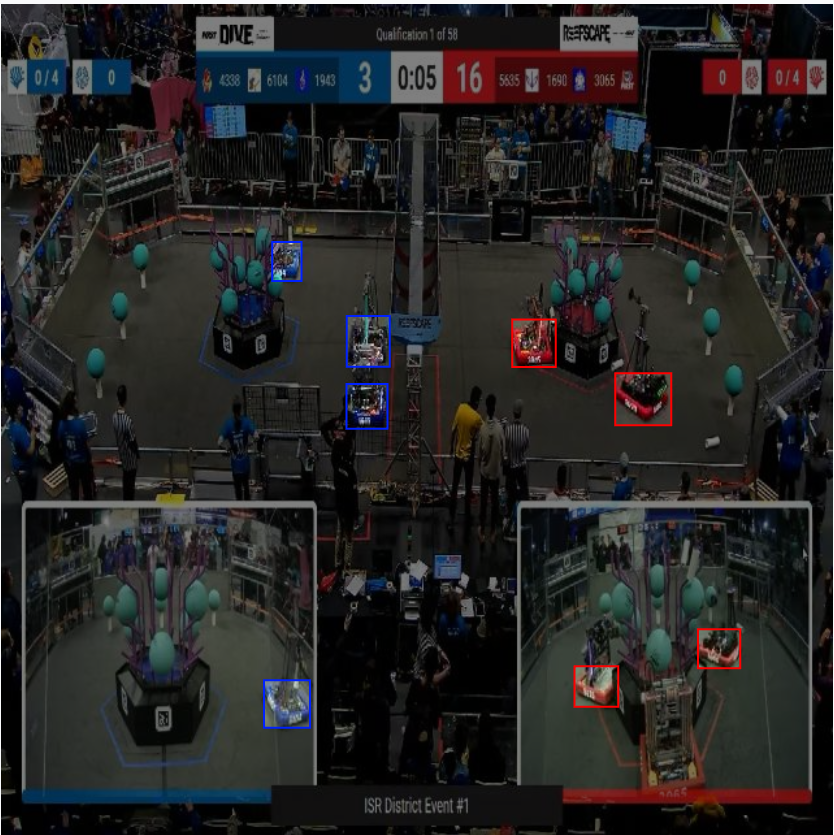
\includegraphics[width=0.7\textwidth]{robots-sample}
  \caption{דוגמה לתיוג רובוטים ובריתות במגרש.}
  \label{fig:robots_sample}
\end{figure}

\begin{figure}[H] \centering
  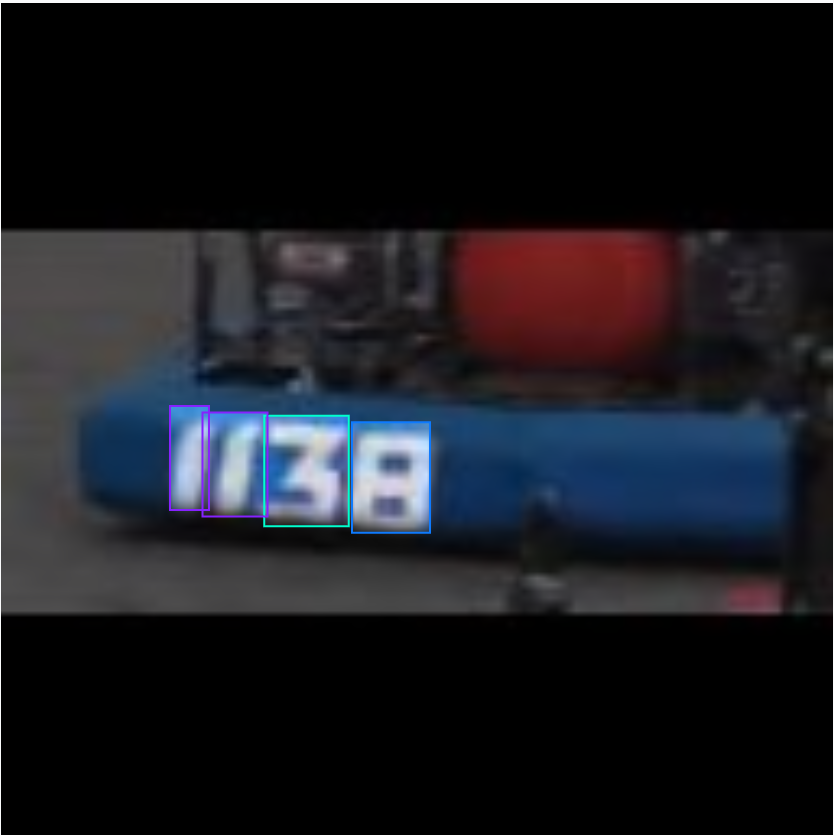
\includegraphics[width=0.5\textwidth]{digits-sample}
  \caption{דוגמה לתיוג ספרות בודדות על באמפר.}
  \label{fig:digits_sample}
\end{figure}

\subsection{תרשימי אימון ותוצאות} \label{app:training}

\begin{figure}[H] \centering
  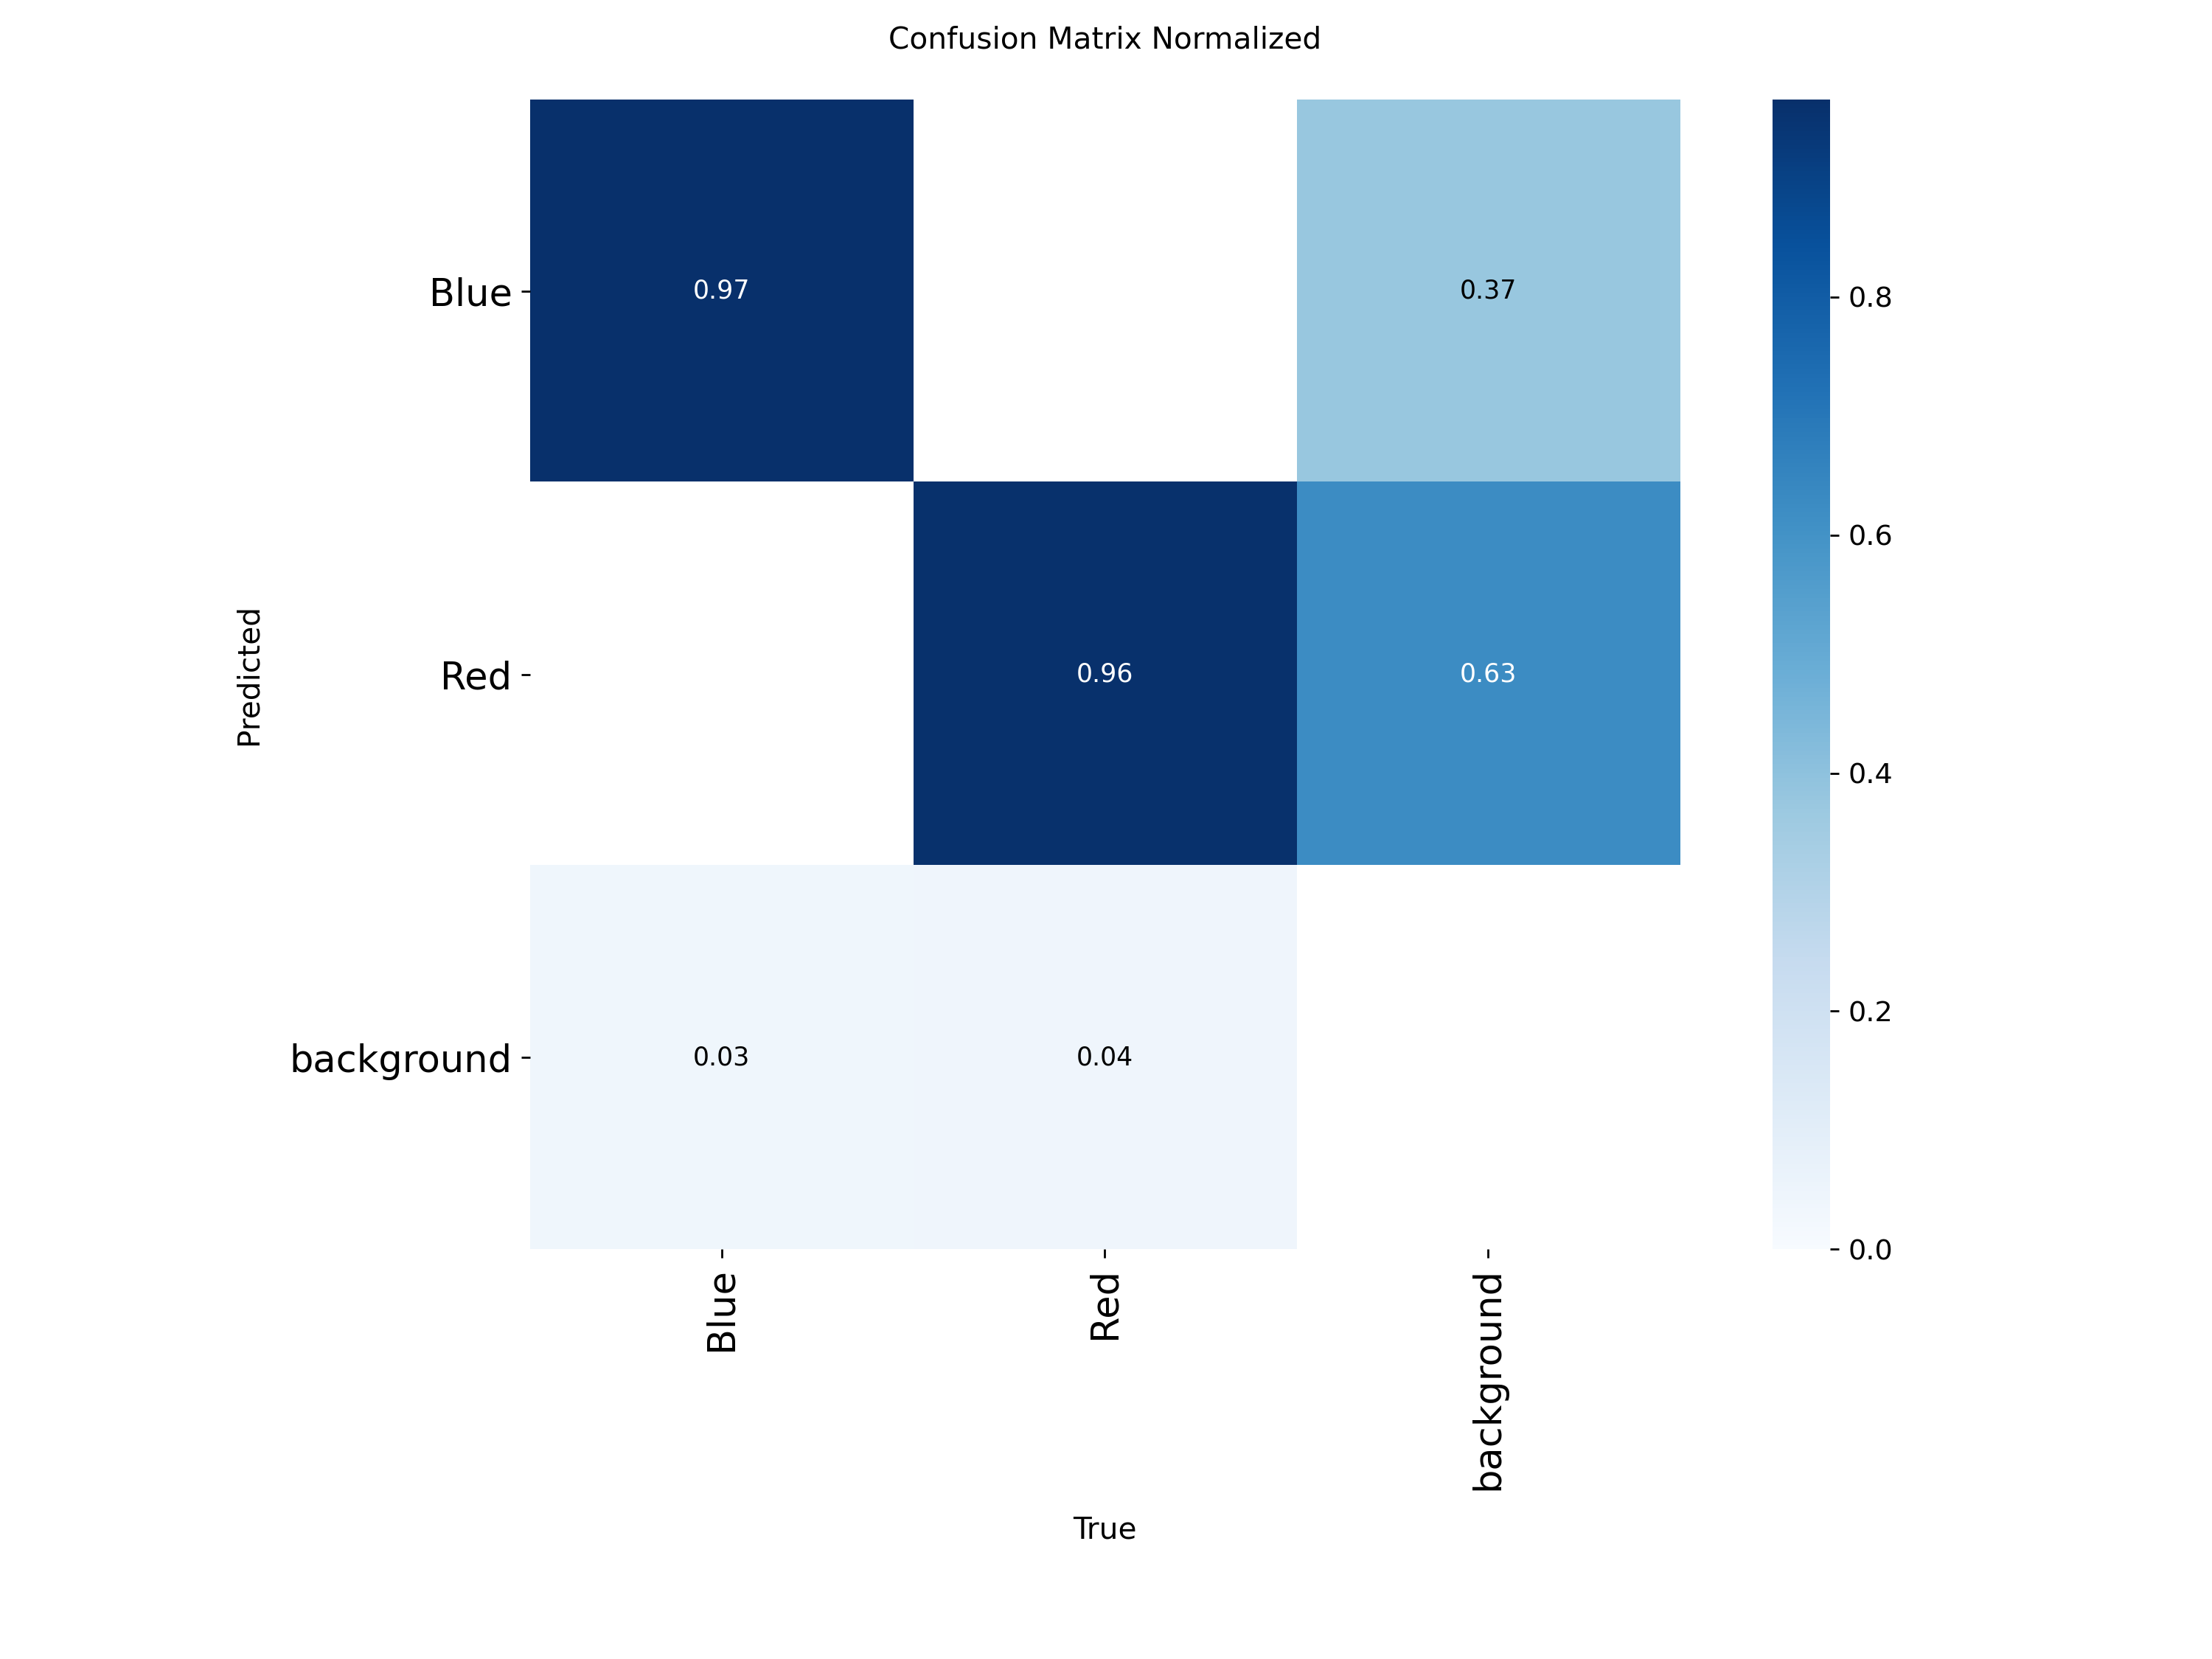
\includegraphics[width=0.8\textwidth]{robots-confusion}
  \caption{מטריצת הבלבול (\textenglish{Confusion Matrix}) של מודל זיהוי הרובוטים.}
  \label{fig:robots_confusion}
\end{figure}

\begin{figure}[H] \centering
  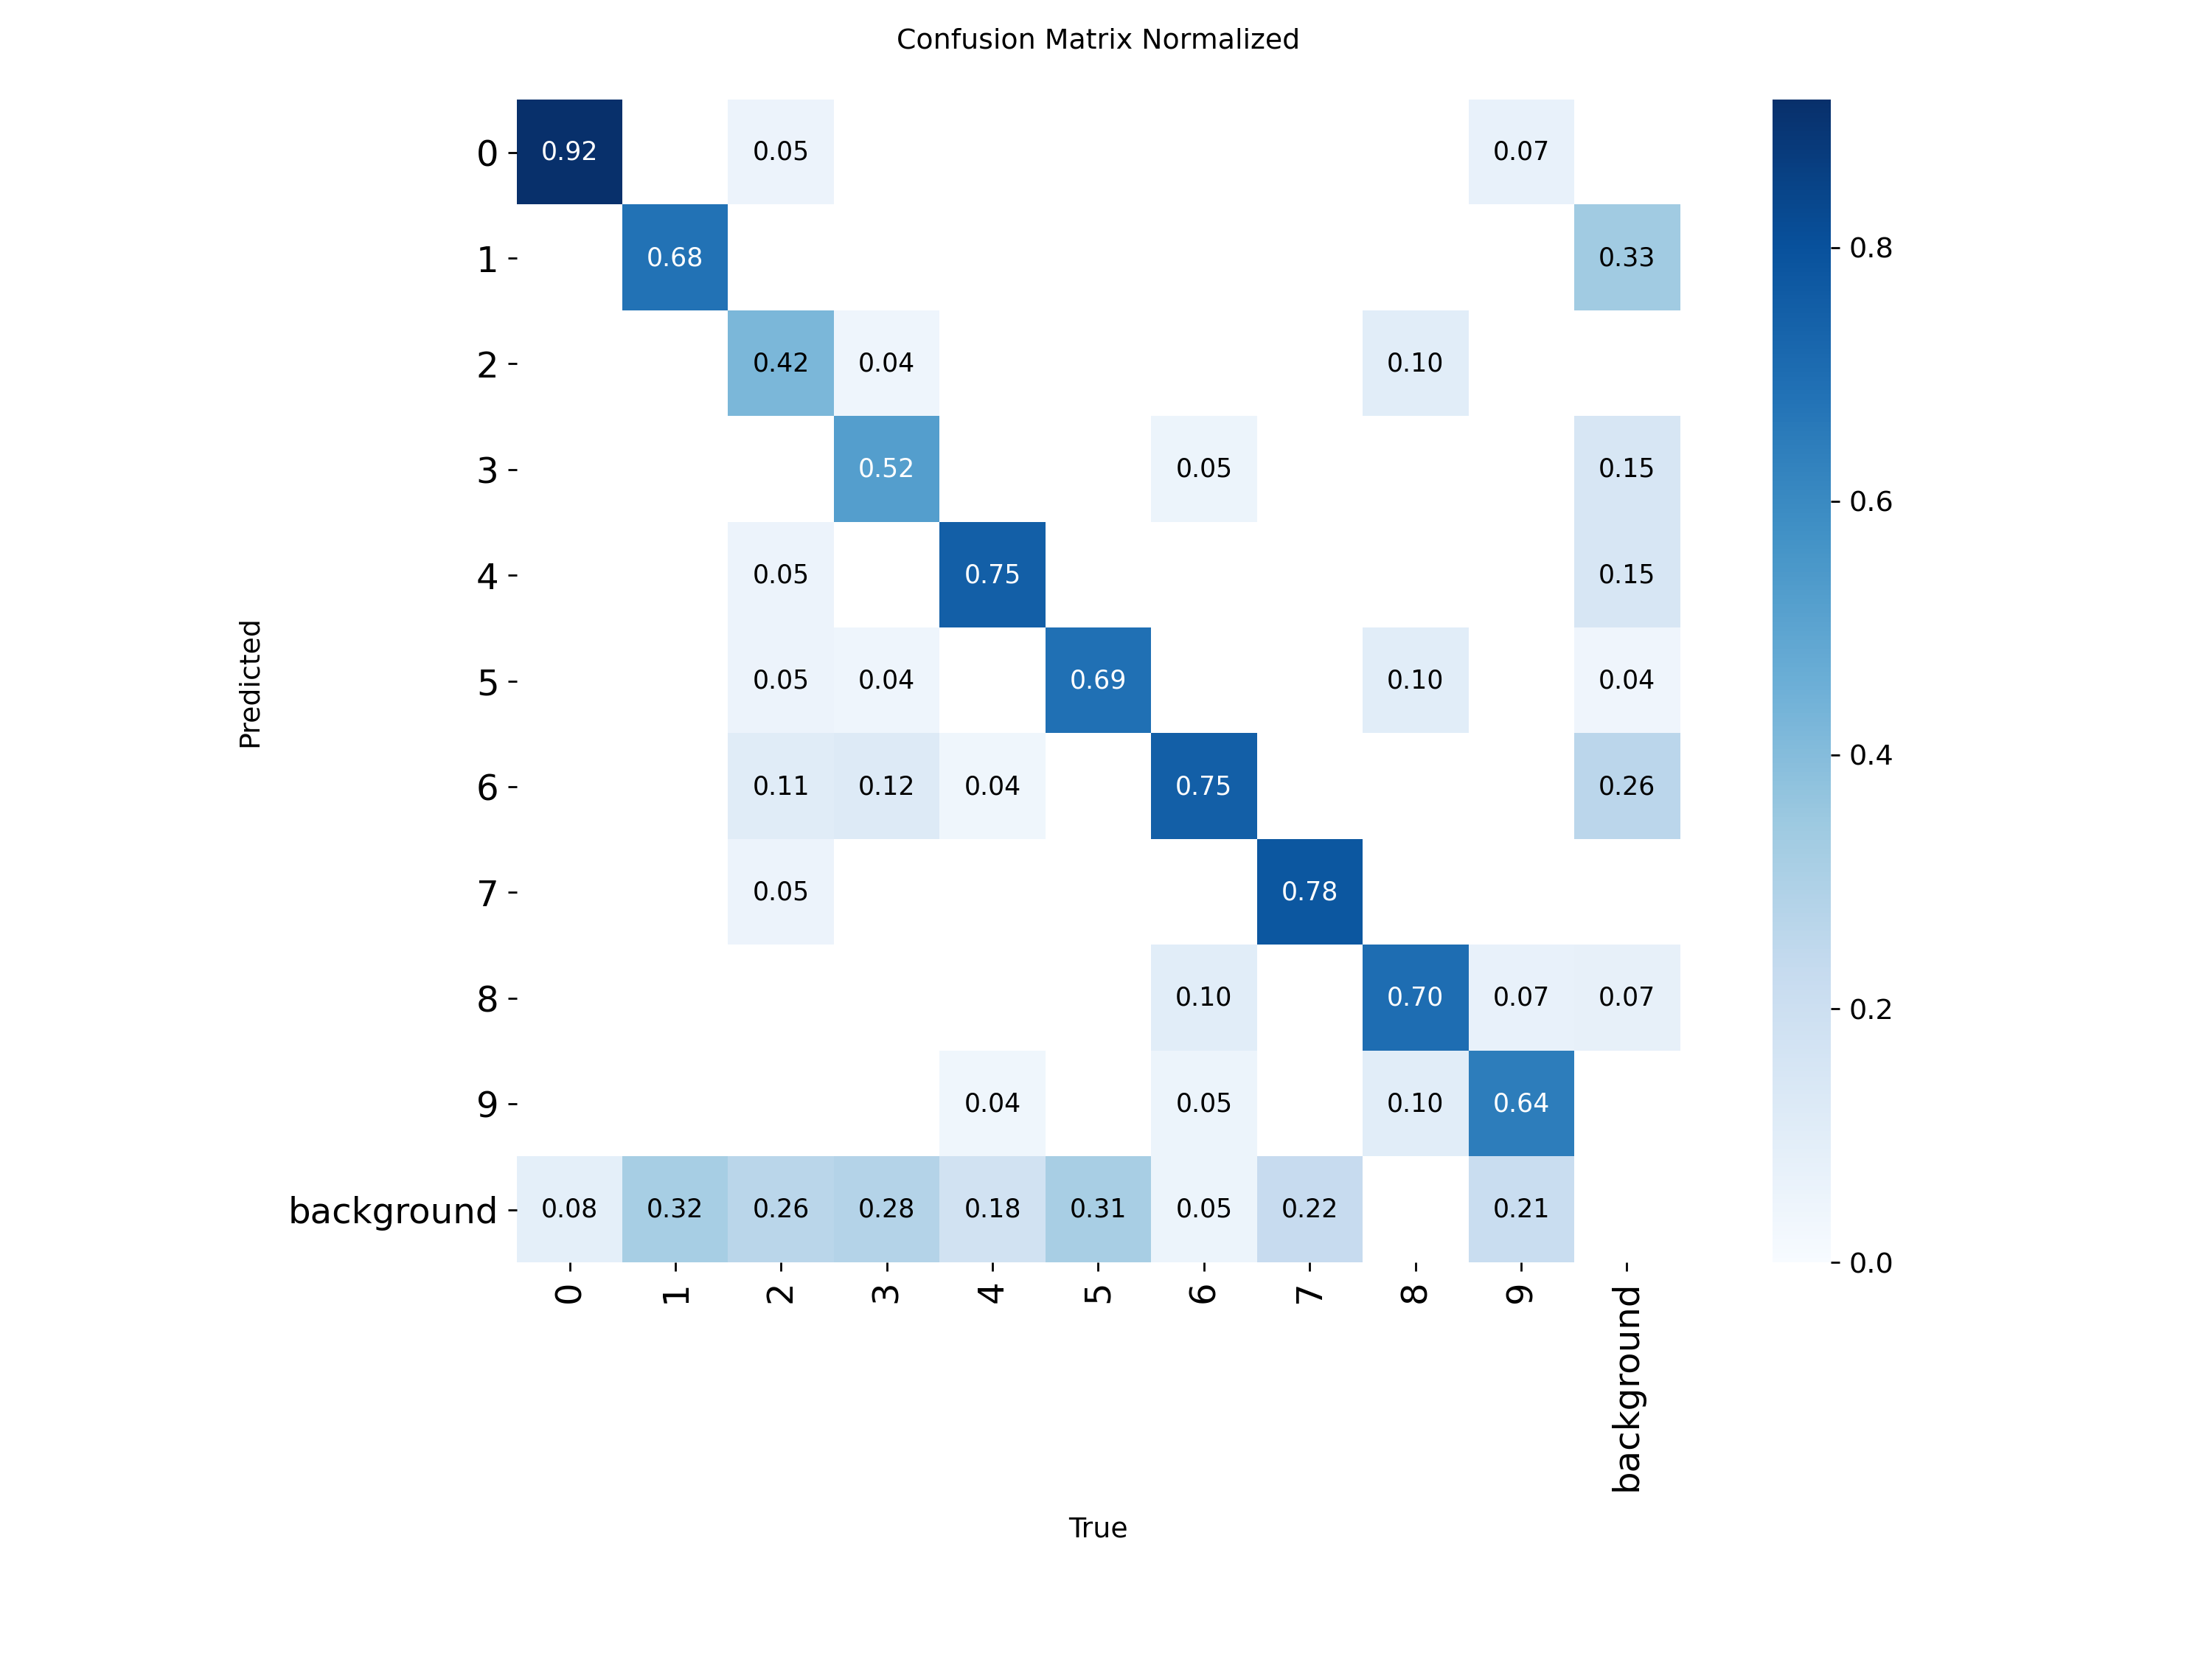
\includegraphics[width=0.8\textwidth]{digits-confusion}
  \caption{מטריצת הבלבול (\textenglish{Confusion Matrix}) של מודל זיהוי הספרות.}
  \label{fig:digits_confusion}
\end{figure}

\begin{table}[H] \centering
  \begin{tabular}{|c|c|c|c|c|c|} \hline
    \textbf{מחלקה} & \textbf{Precision} & \textbf{Recall} & \textbf{mAP@50} & \textbf{mAP@50-95} & \textbf{Support} \\ \hline
    סה''כ & 0.93 & 0.94 & 0.97 &  0.66 & 739 \\ \hline
    כחול & 0.92 & 0.95 & 0.96 & 0.65 & 358 \\ \hline
    אדום & 0.94 & 0.94 & 0.98 & 0.68 & 381 \\ \hline
  \end{tabular}
  \caption{טבלת תוצאות האימון של מודל זיהוי הרובוטים על סט הבדיקה.}
\end{table}

\begin{table}[H] \centering
  \begin{tabular}{|c|c|c|c|c|c|} \hline
    \textbf{מחלקה} & \textbf{Precision} & \textbf{Recall} & \textbf{mAP@50} & \textbf{mAP@50-95} & \textbf{Support} \\ \hline
    סה''כ & 0.75 & 0.78 & 0.85 & 0.43 & 90 \\ \hline
    0 & 0.65 & 0.83 & 0.92 & 0.44 & 6 \\ \hline
    1 & 0.87 & 0.75 & 0.88 & 0.41 & 18 \\ \hline
    2 & 0.68 & 0.71 & 0.79 & 0.41 & 6 \\ \hline
    3 & 0.78 & 0.88 & 0.91 & 0.44 & 8 \\ \hline
    4 & 0.80 & 0.86 & 0.86 & 0.44 & 7 \\ \hline
    5 & 0.80 & 1.0 & 0.93 & 0.54 & 13 \\ \hline
    6 & 0.89 & 0.69 & 0.90 & 0.44 & 12 \\ \hline
    7 & 0.84 & 0.63 & 0.90 & 0.45 & 8 \\ \hline
    8 & 0.65 & 0.48 & 0.58 & 0.22 & 8 \\ \hline
    9 & 0.55 & 0.94 & 0.83 & 0.54 & 4 \\ \hline
  \end{tabular}
  \caption{טבלת תוצאות האימון של מודל זיהוי הספרות על סט הבדיקה.}
\end{table}

\subsection{דוגמאות הצלחה וויזואליות} \label{app:success}

\begin{figure}[H]
  \centering
  \begin{subfigure}[b]{0.9\textwidth}
    \centering
    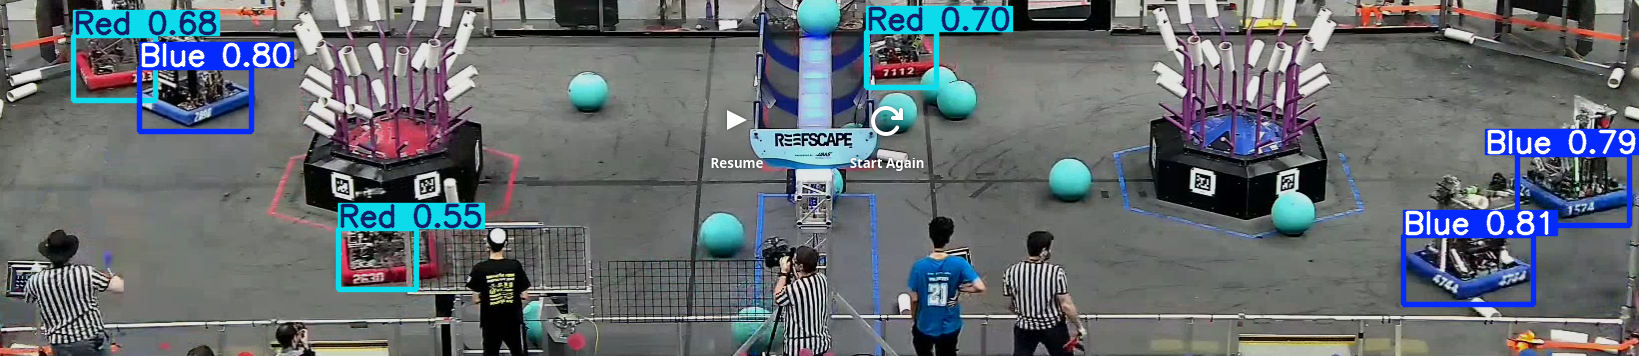
\includegraphics[width=\textwidth]{robots-success-occluded}
    \caption{זיהוי רובוטים מוסתרים חלקית}
  \end{subfigure}
  \begin{subfigure}[b]{0.9\textwidth}
    \centering
    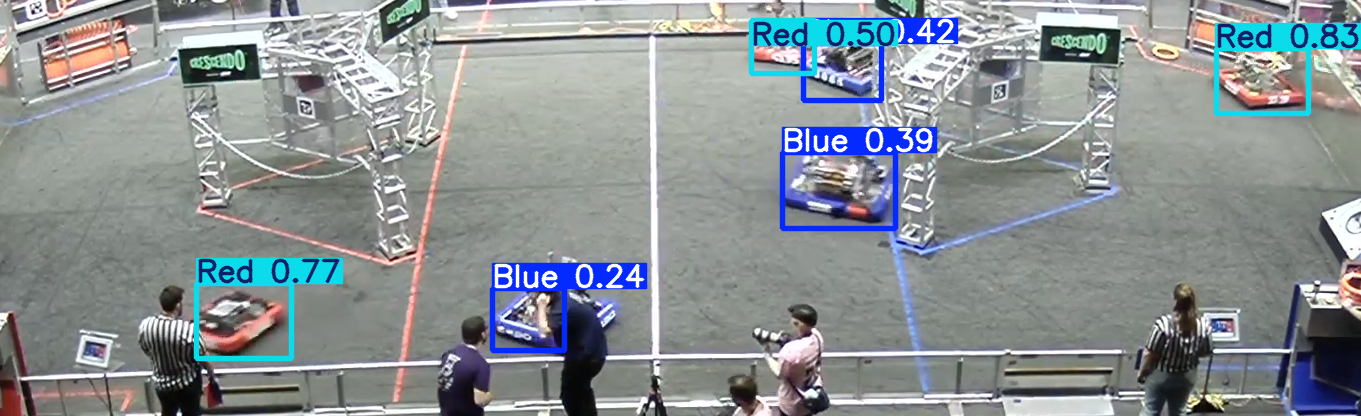
\includegraphics[width=\textwidth]{robots-success-blur}
    \caption{זיהוי רובוטים בתנועה מהירה}
  \end{subfigure}
  \hfill
  \begin{subfigure}[b]{0.45\textwidth}
    \centering
    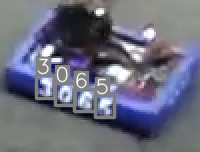
\includegraphics[width=\textwidth]{digits-success-lowres}
    \caption{זיהוי ספרות ברזולוציה נמוכה}
  \end{subfigure}
  \begin{subfigure}[b]{0.45\textwidth}
    \centering
    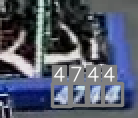
\includegraphics[width=\textwidth]{digits-success-partcrop}
    \caption{זיהוי ספרות על רובוט חתוך חלקית}
  \end{subfigure}
  \caption{דוגמאות להצלחות בזיהויי רובוטים וספרות}
  \label{fig:success}
\end{figure}

\section{ביבליוגרפיה}
\begin{enumerate}[leftmargin=*]

  \begin{english}

  \item Ultralytics. (2025). Ultralytics YOLO26. Ultralytics Docs. \\
    \href{https://docs.ultralytics.com/models/yolo26/}{https://docs.ultralytics.com/models/yolo26/}

  \item Jocher, G., \& Qiu, J. (2026). Ultralytics YOLO26
    (Version 1.0.0) [Computer software]. \\
    \href{https://github.com/ultralytics/ultralytics}{https://github.com/ultralytics/ultralytics}

  \item Zhang, Y., Sun, P., Jiang, Y., Yu, D., Weng, F.,
    Yuan, Z., Luo, P., Liu, W., \& Wang, X. (2022).
    ByteTrack: Multi-Object Tracking by Associating Every Detection Box.
    Proceedings of the European Conference on Computer Vision (ECCV). \\
    \href{https://arxiv.org/abs/2110.06864}{https://arxiv.org/abs/2110.06864}

  \item Tiangolo, S. (2018). FastAPI framework, high performance,
    easy to learn, fast to code, ready for production [Computer software]. \\
    \href{https://github.com/fastapi/fastapi}{https://github.com/fastapi/fastapi}

  \item Navarro, G. (2001). A guided tour to approximate string matching.
    ACM Computing Surveys, 33(1), 31--88. \\
    \href{https://doi.org/10.1145/375360.375365}{https://doi.org/10.1145/375360.375365}

  \end{english}

\end{enumerate}


\end{document}
